\documentclass[conf]{new-aiaa}
%\documentclass[journal]{new-aiaa} for journal papers
\usepackage[utf8]{inputenc}

\usepackage{graphicx}
\usepackage{amsmath}
\usepackage{commath}
\usepackage[version=4]{mhchem}
\usepackage{siunitx}
\usepackage{longtable,tabularx}
\usepackage{float}
\usepackage{listings}
\usepackage{pdfpages}
\usepackage{color} %red, green, blue, yellow, cyan, magenta, black, white
\definecolor{mygreen}{RGB}{28,172,0} % color values Red, Green, Blue
\definecolor{mylilas}{RGB}{170,55,241}
\setlength\LTleft{0pt} 

\lstset{language=Matlab,%
	basicstyle=\footnotesize,
	breaklines=true,%
	morekeywords={matlab2tikz},
	keywordstyle=\color{blue},%
	morekeywords=[2]{1}, keywordstyle=[2]{\color{black}},
	identifierstyle=\color{black},%
	stringstyle=\color{mylilas},
	commentstyle=\color{mygreen},%
	showstringspaces=false,%without this there will be a symbol in the places where there is a space
	numbers=left,%
	numberstyle={\tiny \color{black}},% size of the numbers
	numbersep=9pt, % this defines how far the numbers are from the text
	emph=[1]{for,end,break},emphstyle=[1]\color{red}, %some words to emphasise
	%emph=[2]{word1,word2}, emphstyle=[2]{style},    
}

% ================================================================ % 
\title{ASE 389P.4 Methods of Orbit Determination \\ Term Project}

\author{Junette Hsin}
\affil{Masters Student, Aerospace Engineering and Engineering Mechanics, University of Texas, Austin, TX 78712}

\begin{document}

\maketitle

\begin{abstract}
	The theory and algorithms are derived and computer program to establish the trajectory of
	an Earth-orbiting satellite is developed. The assumptions for the study are:
	
	\begin{itemize}
		\item Three tracking stations taking apparent range and range-rate data are available for tracking the	satellite. Apparent quantities imply that the one-way light time between signal transmission and reception were modeled into the measurement (i.e. the effect is dealt with).
		\item The force model used to generate the truth is the EGM96 gravity field of degree and order 20,
		attitude-dependent solar radiation pressure, and atmospheric drag.
		\item The satellite is a box-wing shaped with one Sun-pointed solar panel with known component sizes, material properties, and orientation. The spacecraft -Z axis (in the spacecraft body reference frame) is always Nadir-pointed and has the antenna.
	\end{itemize}
	

\end{abstract}



% ================================================================ % 
\section*{Problem 1}

 % \subsubsection*{Statement} 
\begin{center}
\fbox{Prefit residuals for all data and all sensors.} \\
\end{center}


% ================================================================ % 
\section*{Problem 2}

% \subsubsection*{Statement} 
\begin{center}
	\fbox{ Postfit residuals (bounded by 3-$\sigma$ bounds of the innovations covariance) for all data and all sensors} \\
\end{center}


% ---------------------------------------------------------------- % 
\subsubsection*{Solution for Problems 1 and 2} 

The prefit and postfit residuals for all stations are provided below (all data from all stations were used to filter the best estimate). The postfit residuals mostly lie within the 3-sigma covariance bounds, which are plotted as red lines. 

\begin{center}
	
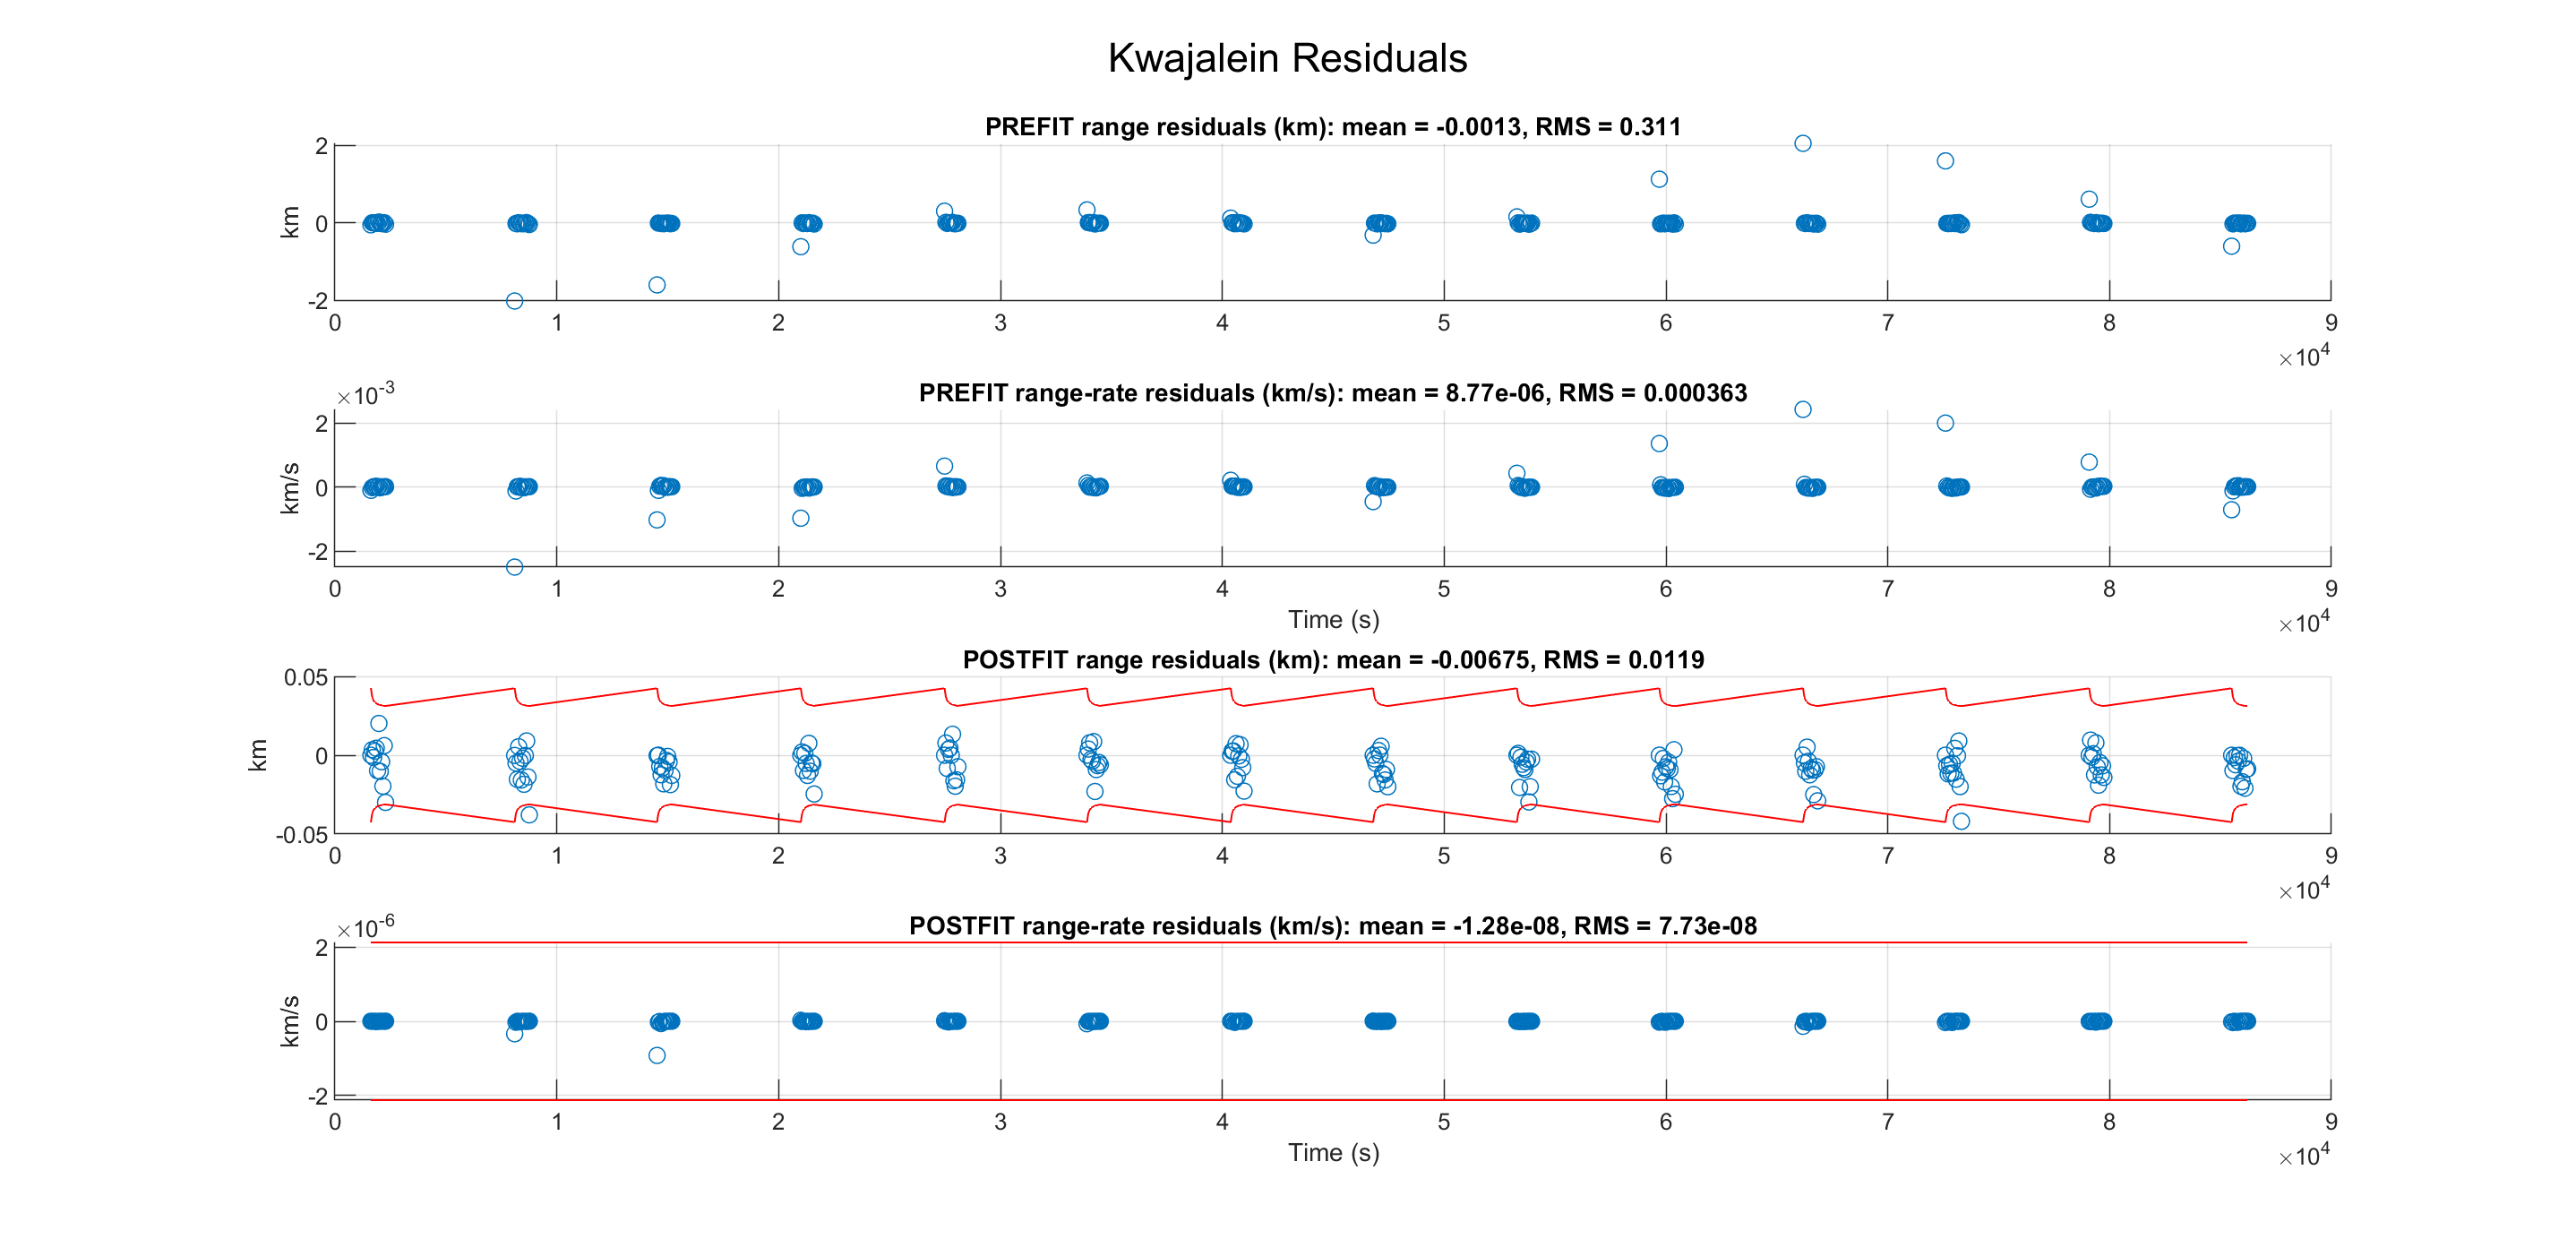
\includegraphics[width=\textwidth]{KJL_res_all.png}

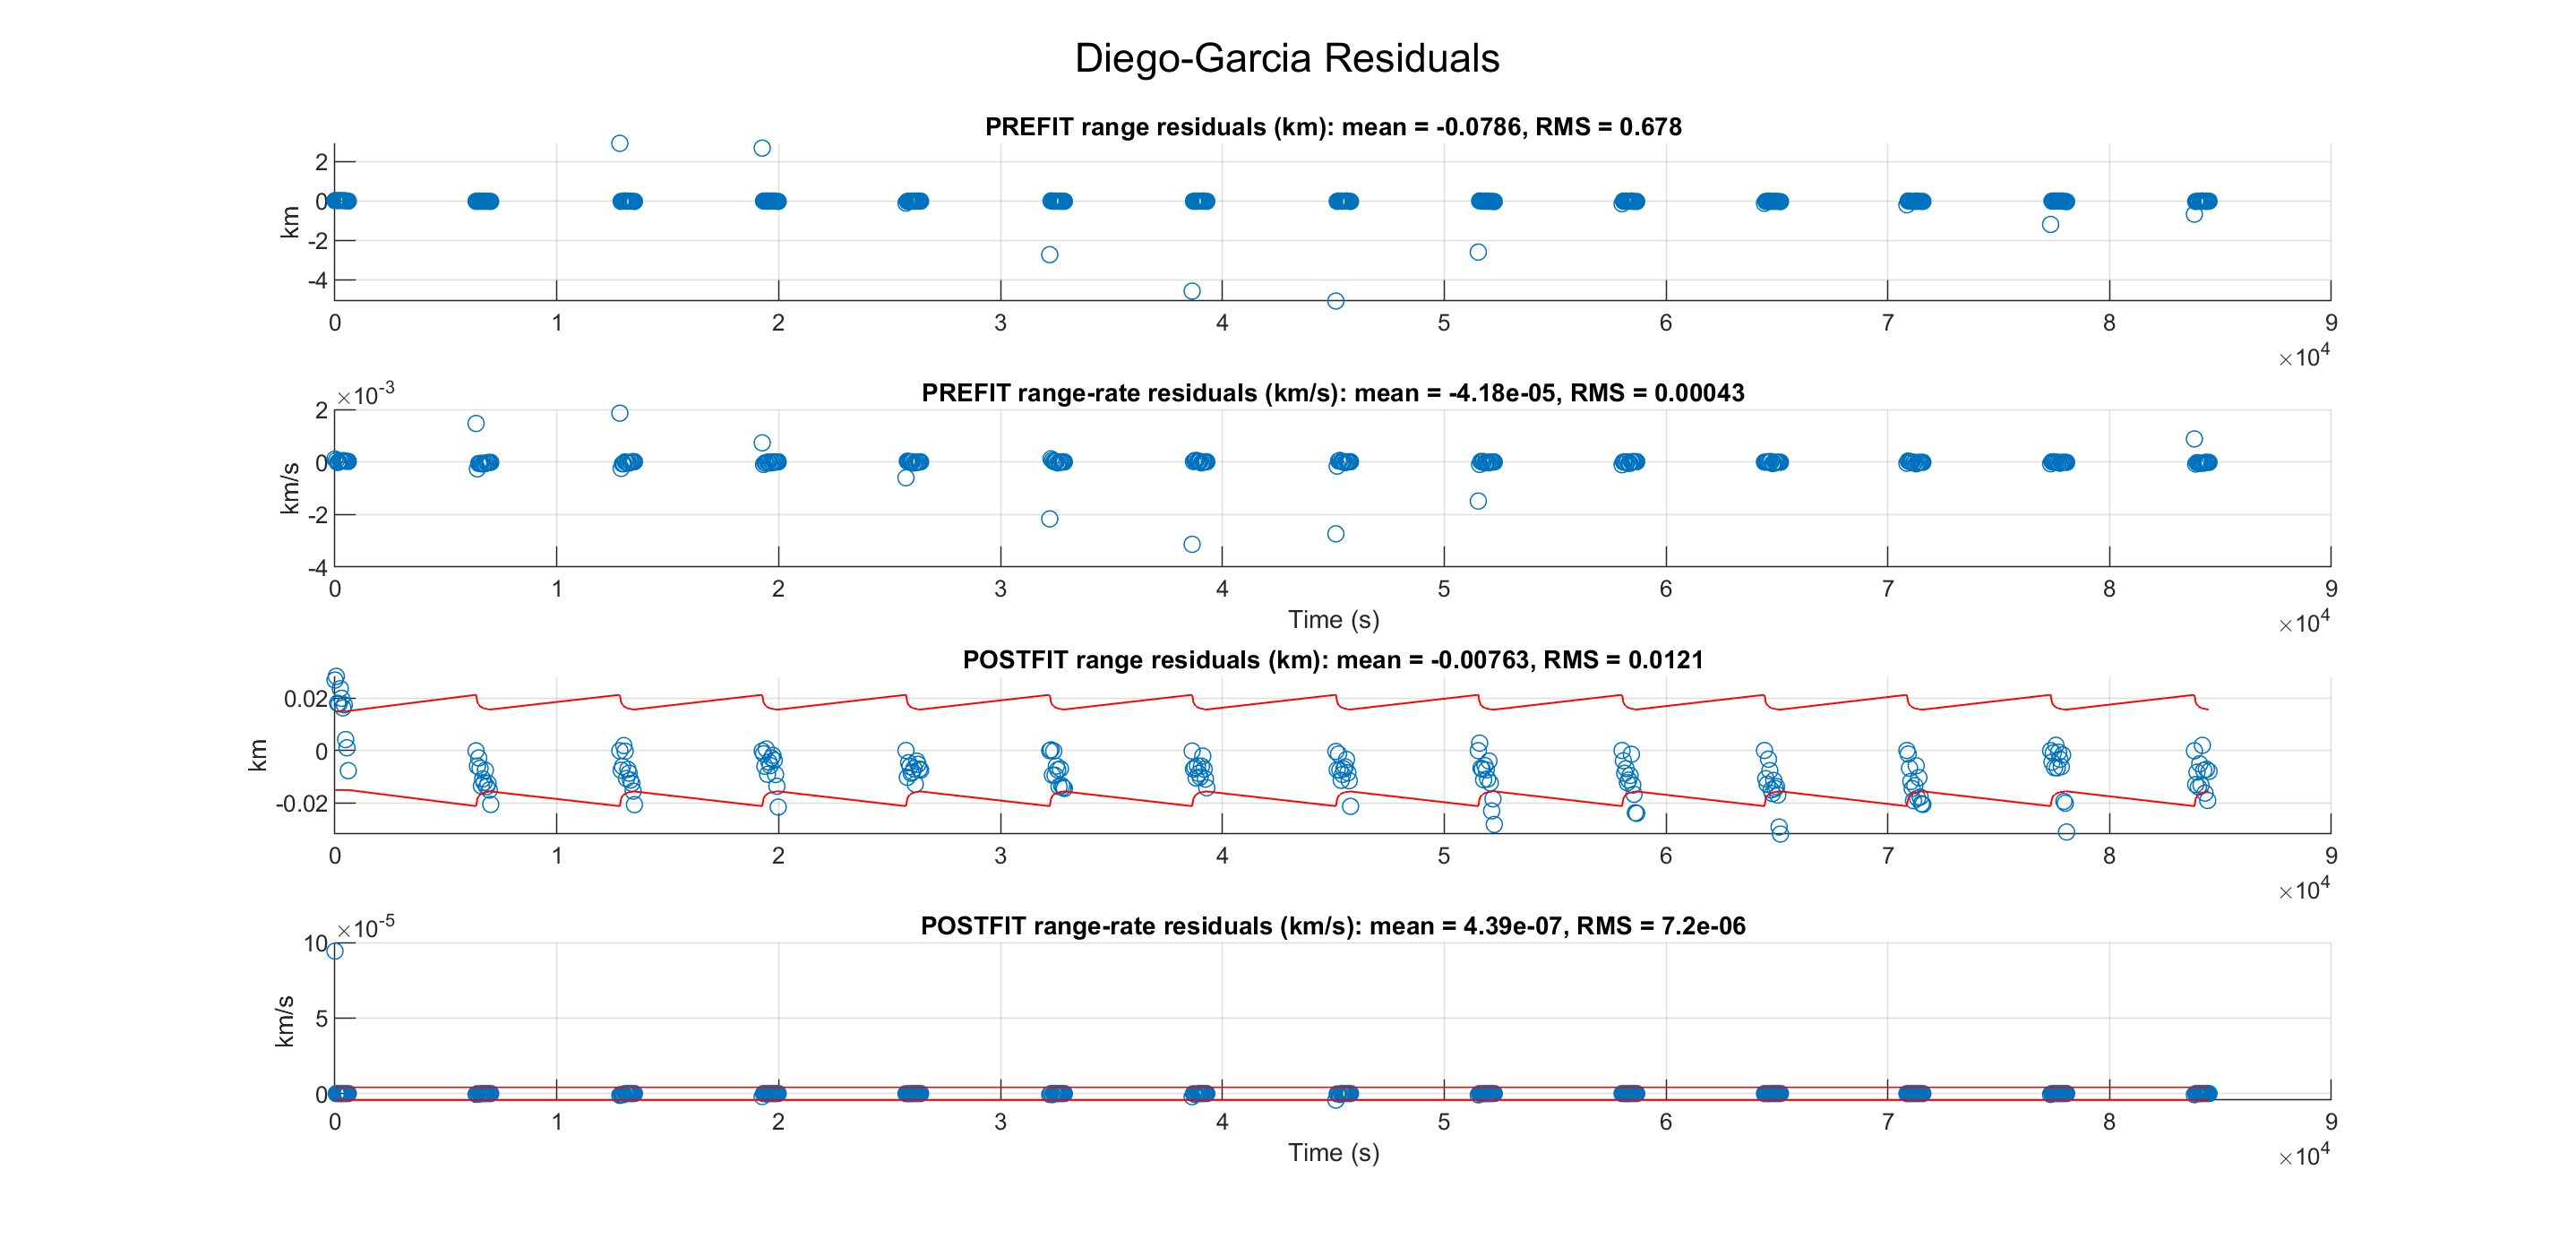
\includegraphics[width=\textwidth]{DGO_res_all.png}

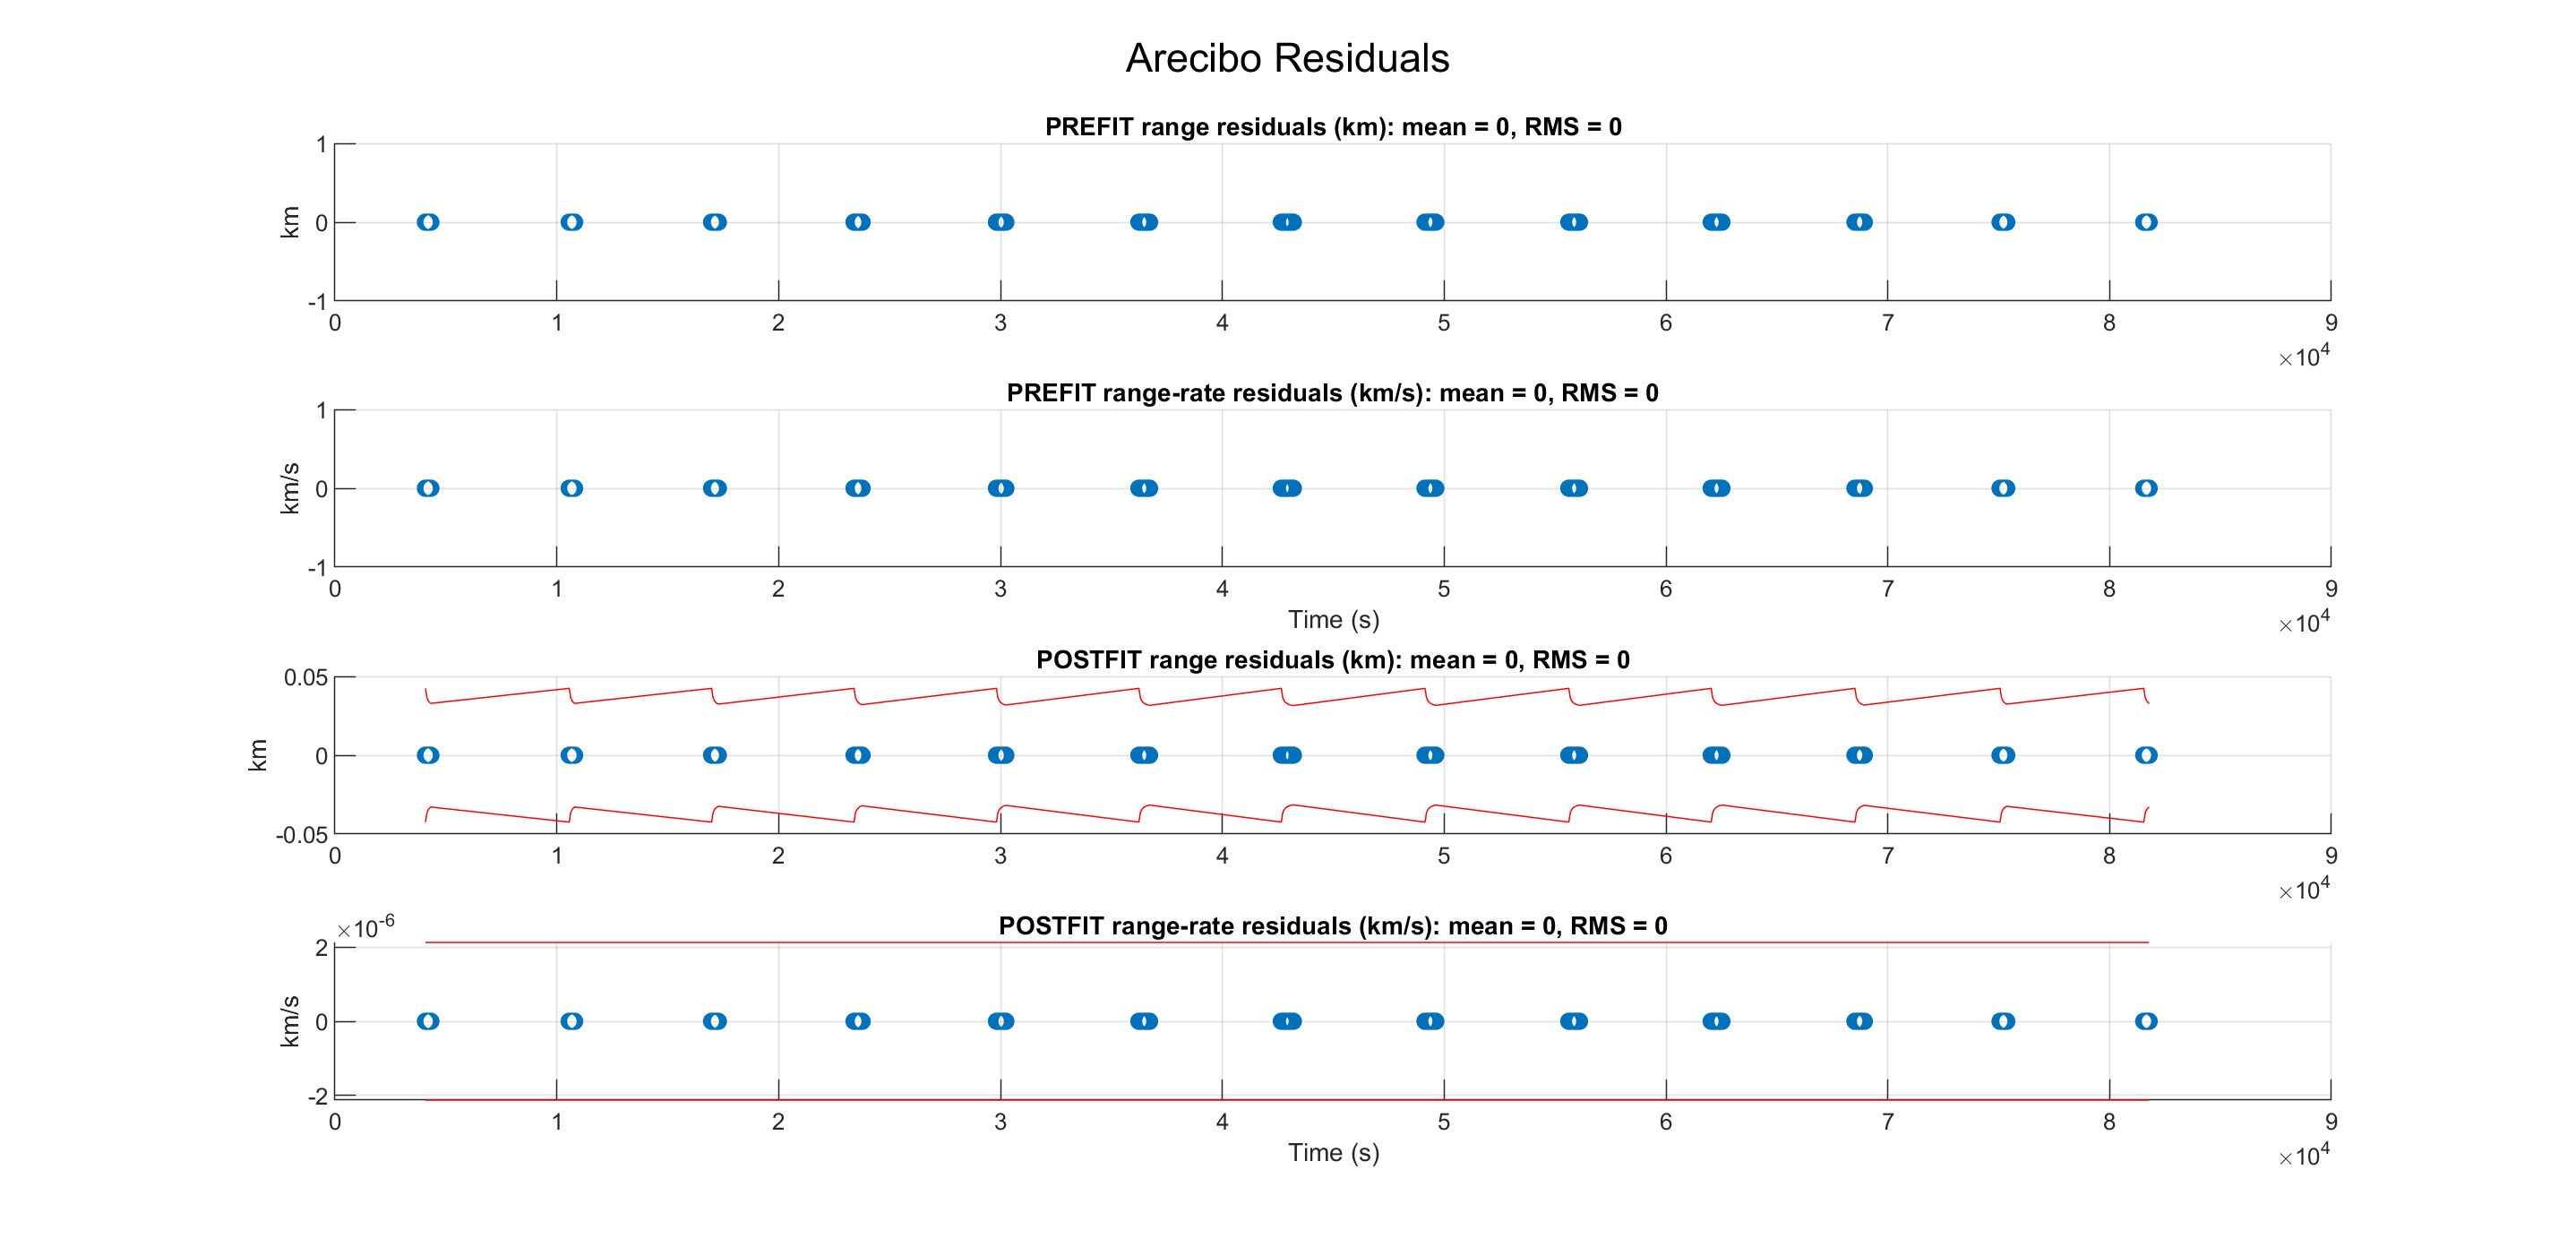
\includegraphics[width=\textwidth]{ACB_res_all.png}

\end{center}

The Diego-Garcia plots have one residual for range-rate which lies far outside the 3-sigma covariance bounds. Zooming in reveals that most of the residuals lie within the 3-sigma covariance bounds, although some residuals 

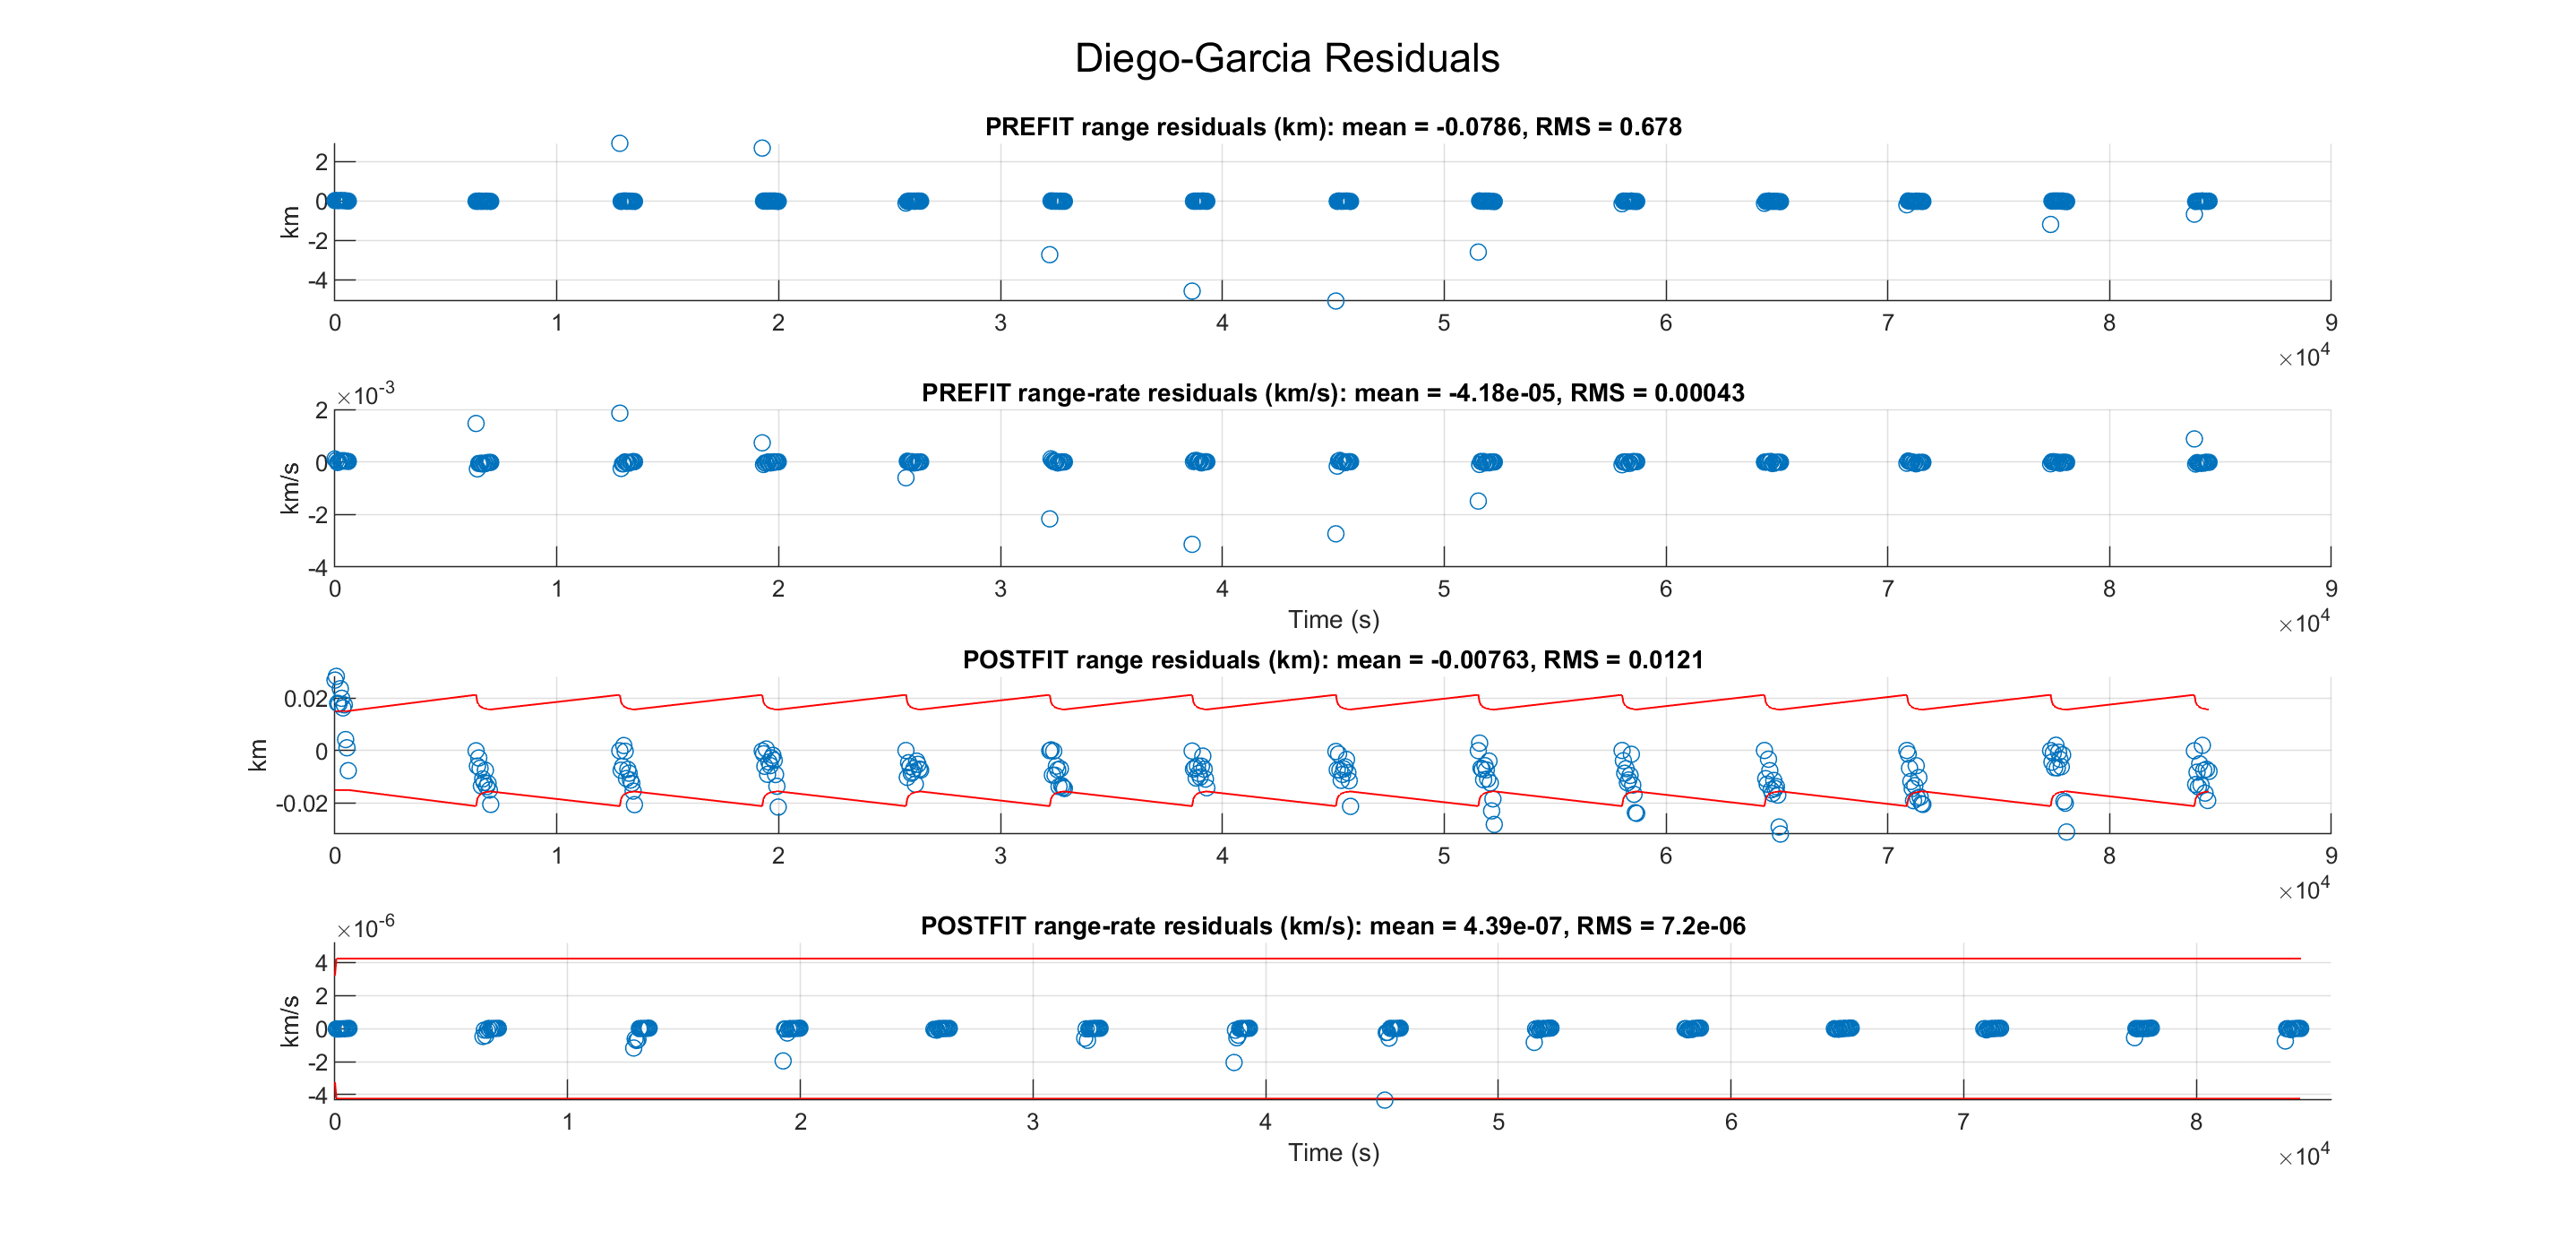
\includegraphics[width=\textwidth]{DGO_res_all_zoom.png}

There seems to be a station bias for Kwajalein and Diego-Garcia, particularly in ranging. For the next phase of the project, I am planning on estimating the bias for each station to remove its effect on the estimation process and the residuals. 

Arecibo residuals have 0 mean and 0 RMS. This is strange to me and I believe there is something going wrong as I expected there to be more noise due to both the estimation process and measurements themselves. When plotting the Arecibo residuals for the range-only (Case A) and range-rate (Case B) simulations, the residuals show some noisy behavior characteristic of sensors. 

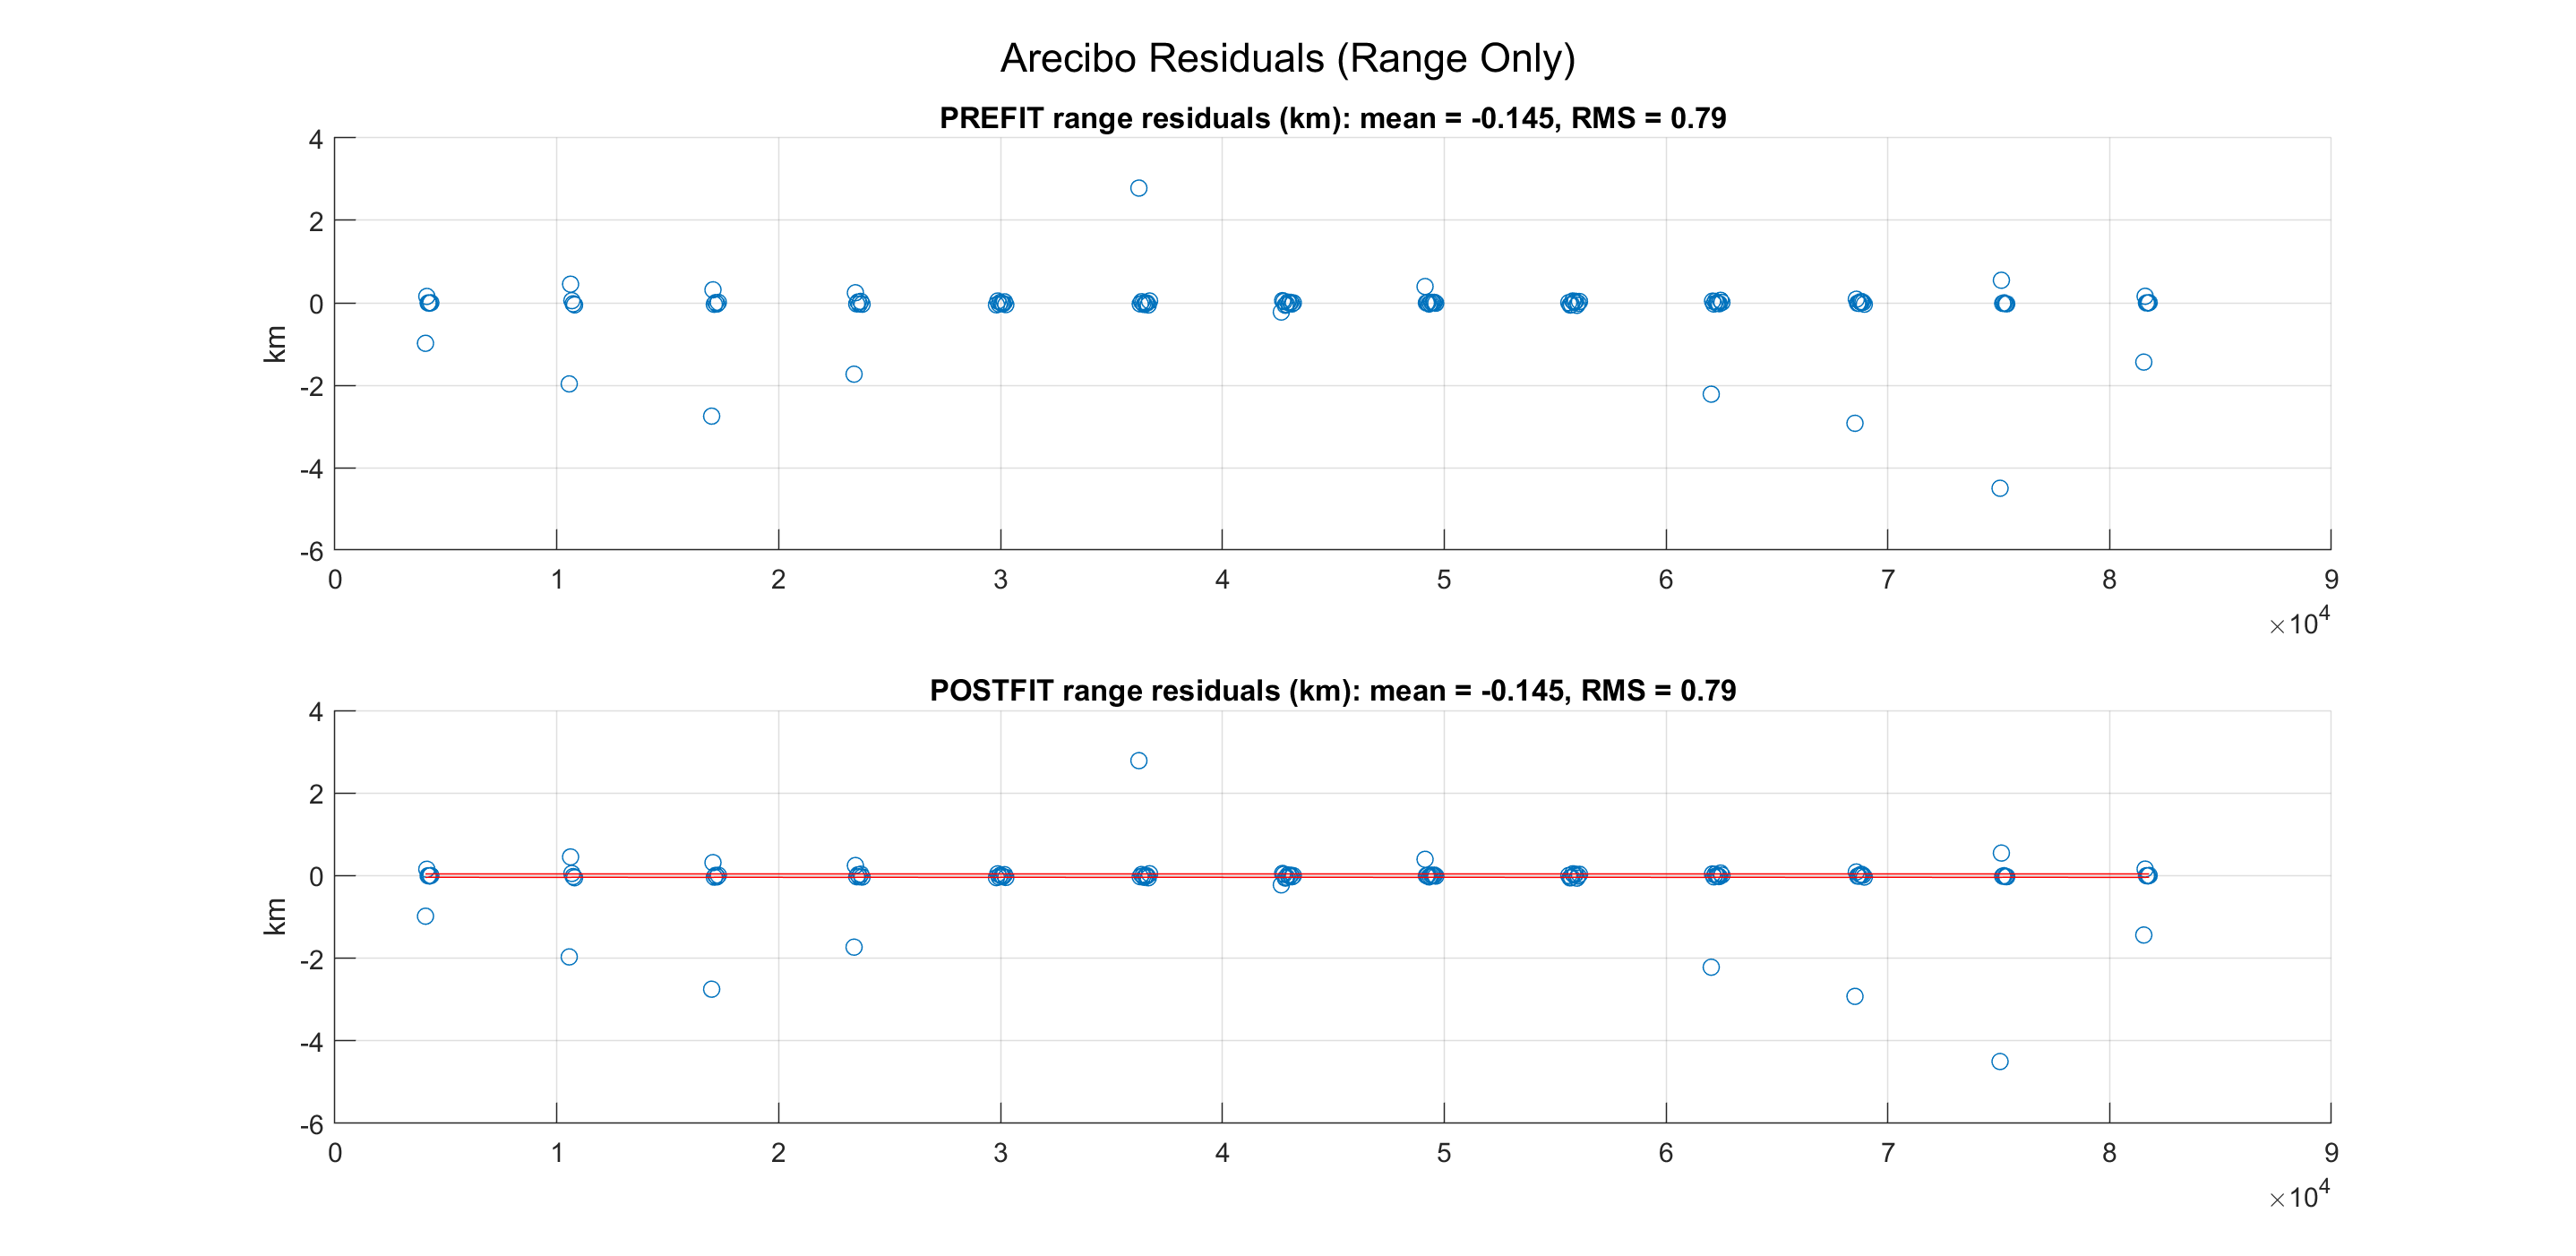
\includegraphics[width=\textwidth]{ACB_res_r.png}

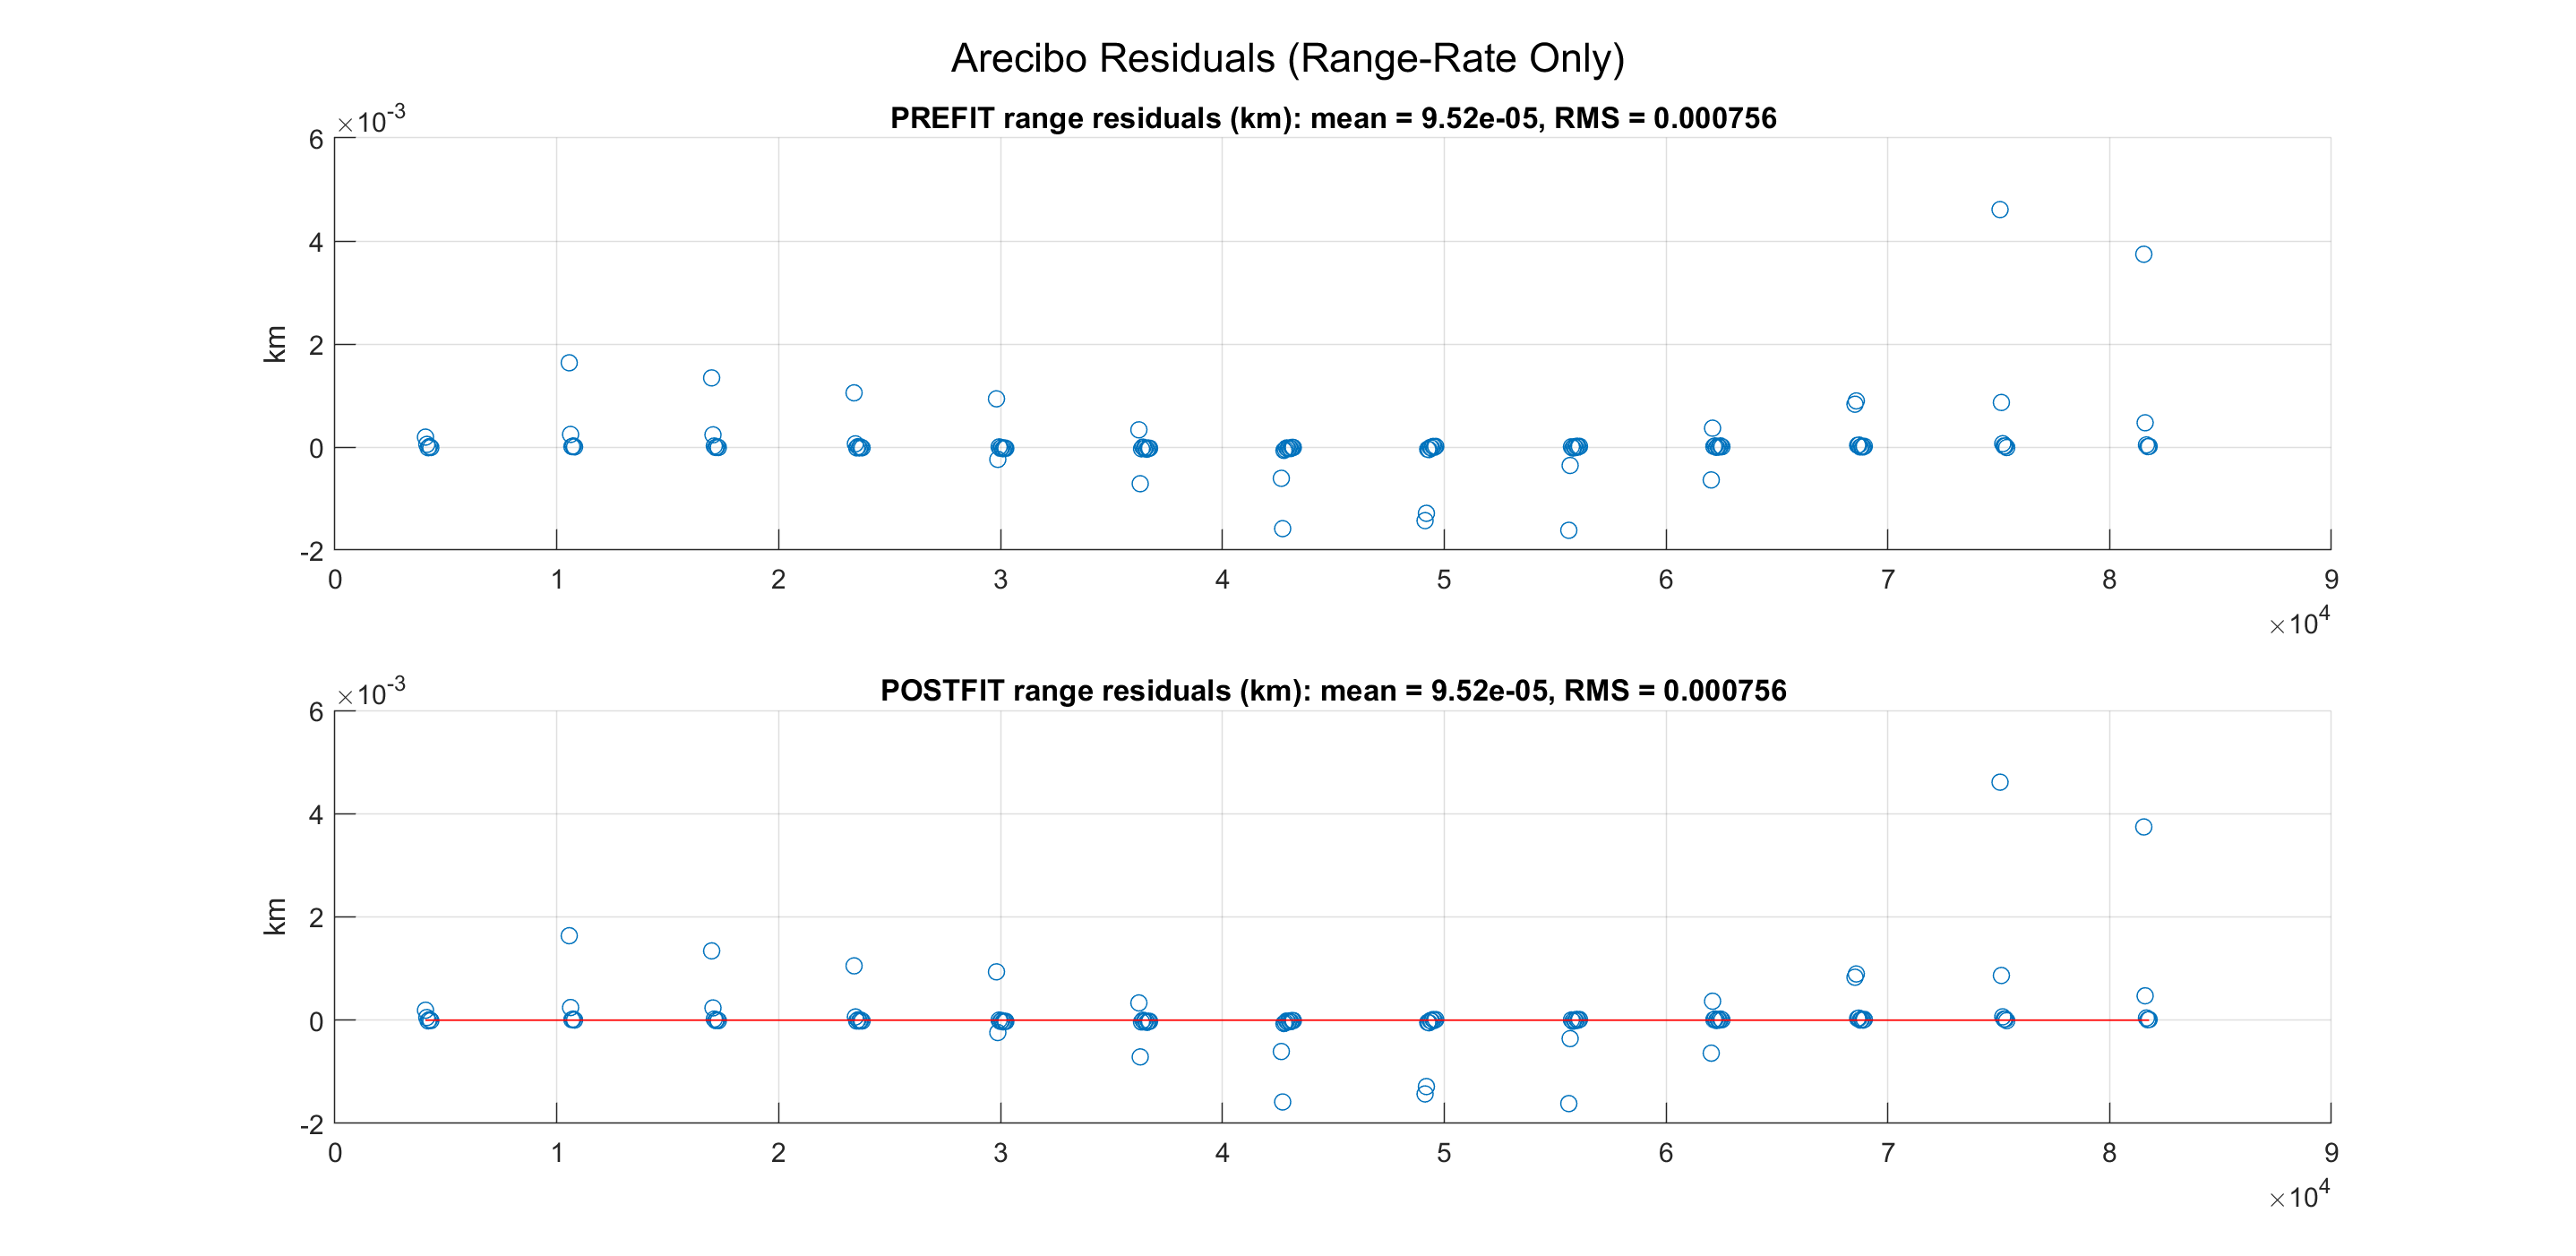
\includegraphics[width=\textwidth]{ACB_res_rr.png}

This warrants further investigation, which I will complete during the next phase of the project. 


% ================================================================ % 
\section*{Problem 3}

% \subsubsection*{Statement} 
\begin{center}
	\fbox{ 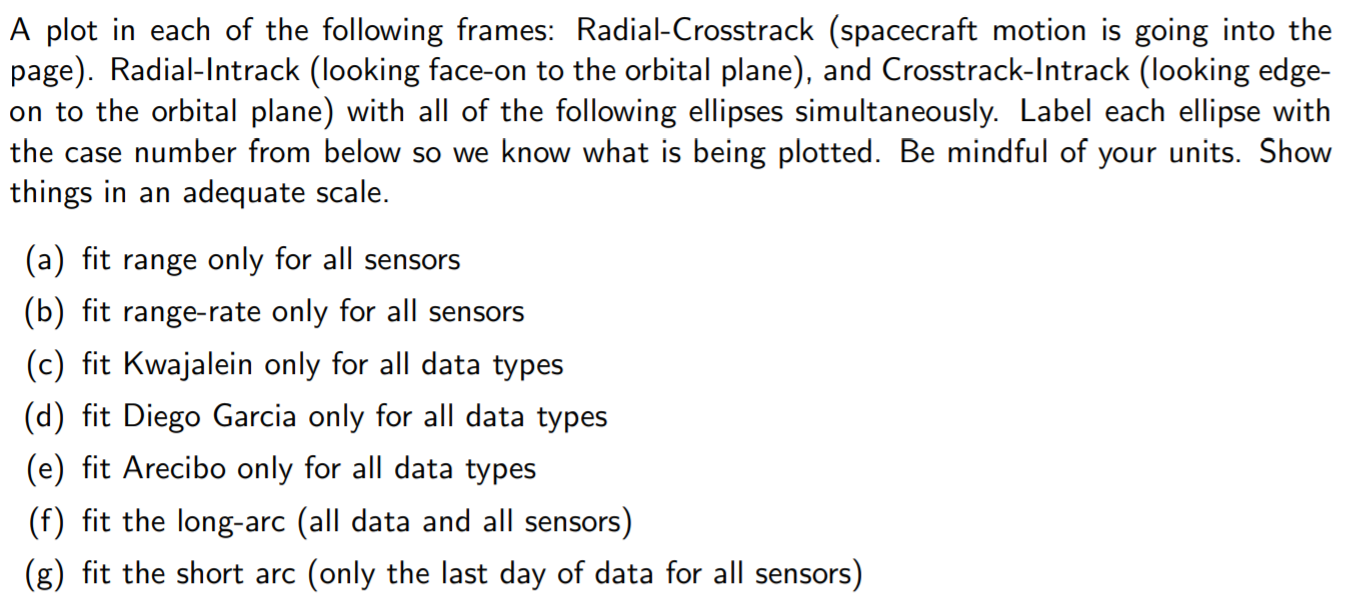
\includegraphics[width=0.8\textwidth]{prob_3.png}}
\end{center}



% ---------------------------------------------------------------- % 
\subsubsection*{Solution} 

The radial-intrack, radial-crosstrack, and intrack-crosstrack plots for Cases A - F are provided below. For Case F, the "long arc" is really just 24 hours for the first phase of this project. \textbf{The units for all axes are in kilometers.}

\begin{center}
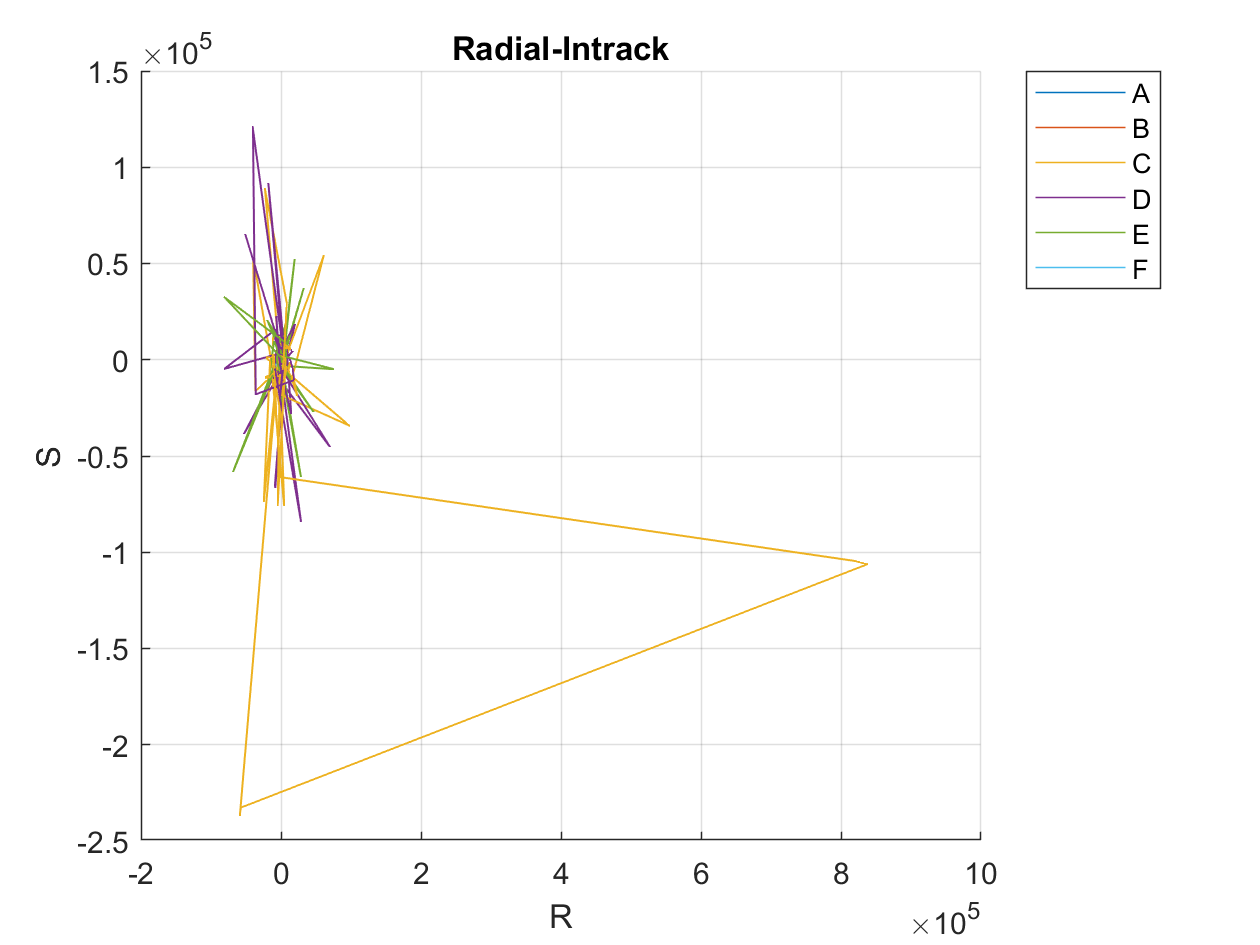
\includegraphics[width=0.6\textwidth]{radial-intrack.png}

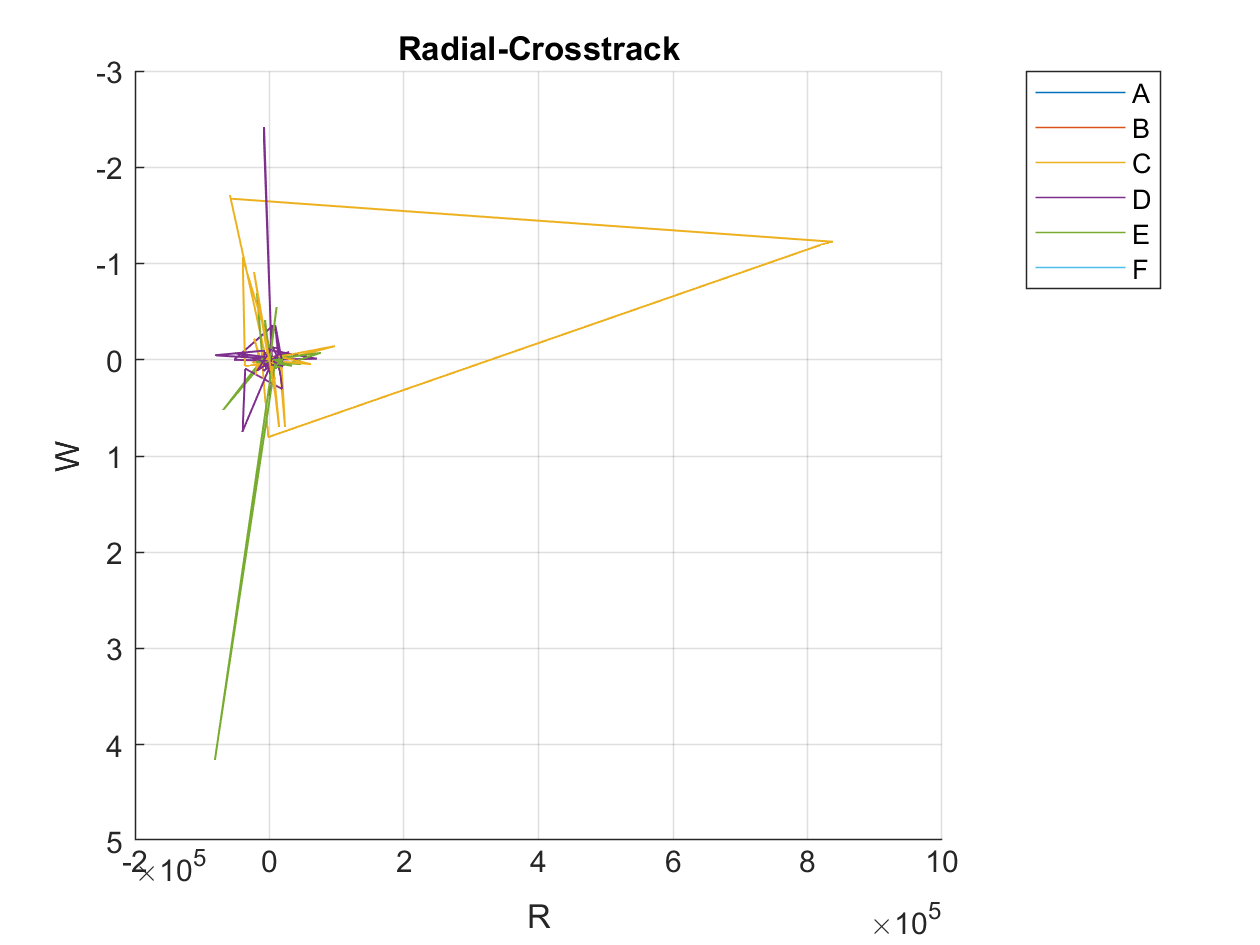
\includegraphics[width=0.6\textwidth]{radial-crosstrack.png}

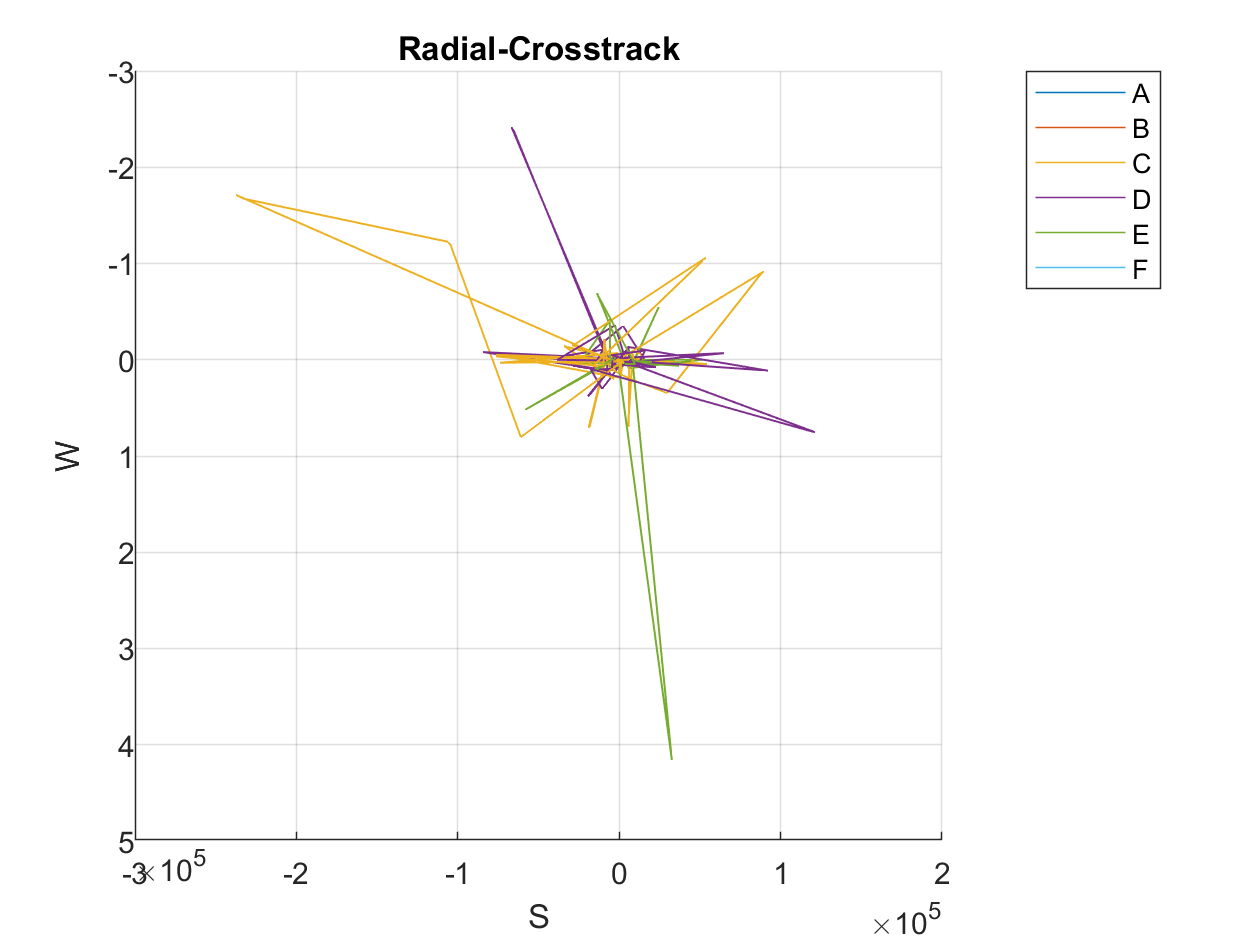
\includegraphics[width=0.6\textwidth]{intrack-crosstrack.png}
\end{center}

Cases C, D, and E were poorly fit with only one station data. When Cases C, D, and E are removed, the ellipses of each orbit are possible to recognize:  

\begin{center}
	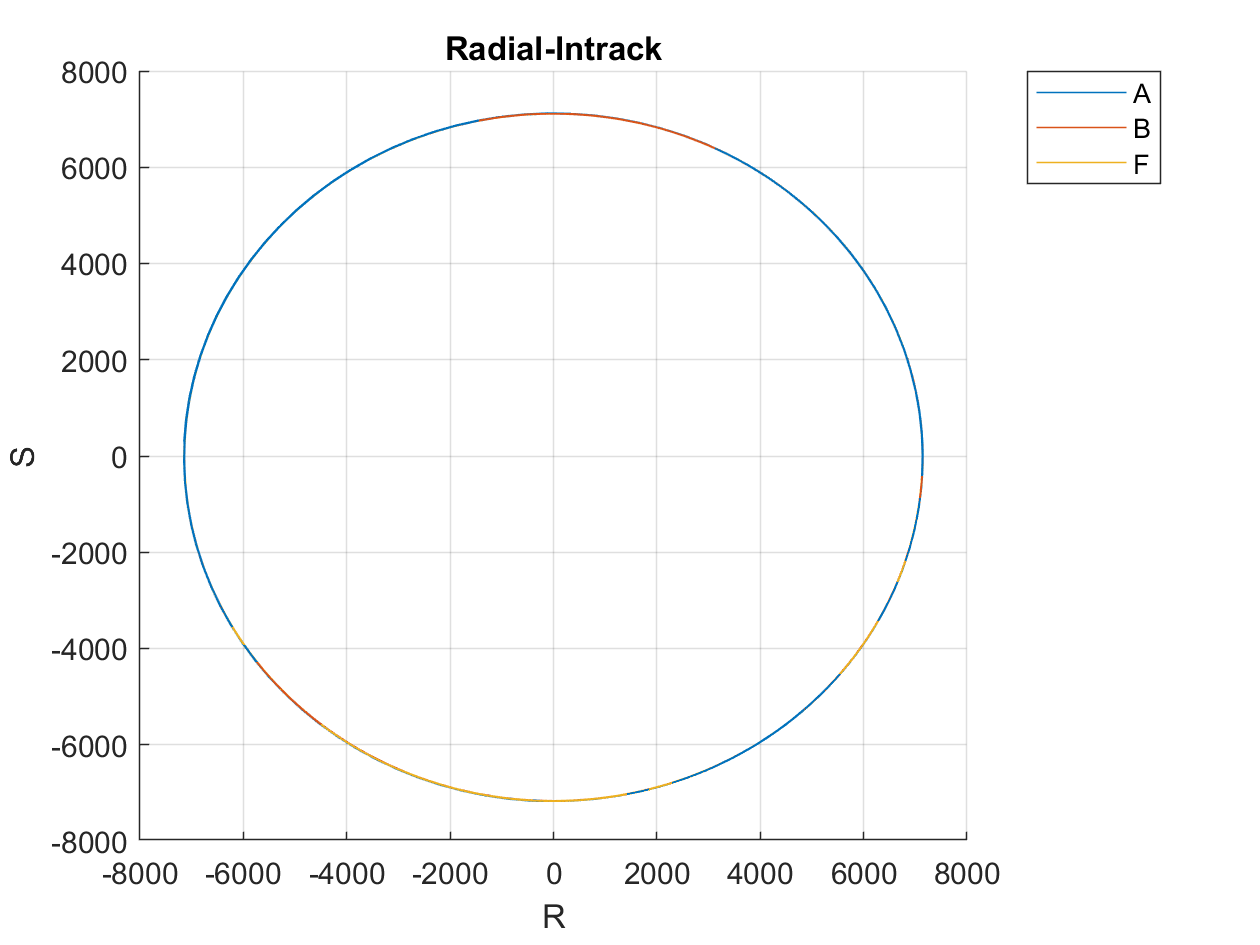
\includegraphics[width=0.6\textwidth]{radial-intrackABF.png}
	
	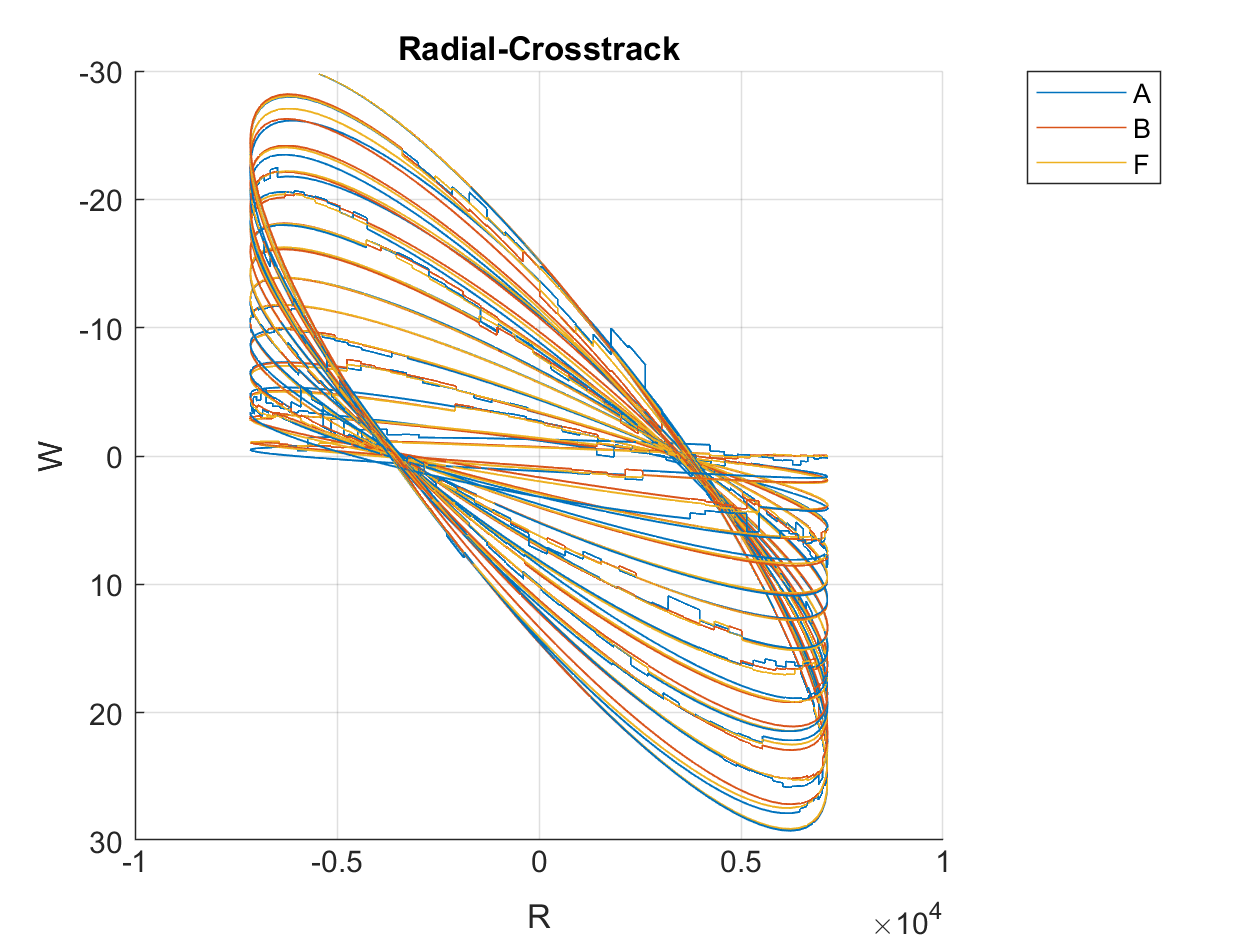
\includegraphics[width=0.6\textwidth]{radial-crosstrackABF.png}
	
	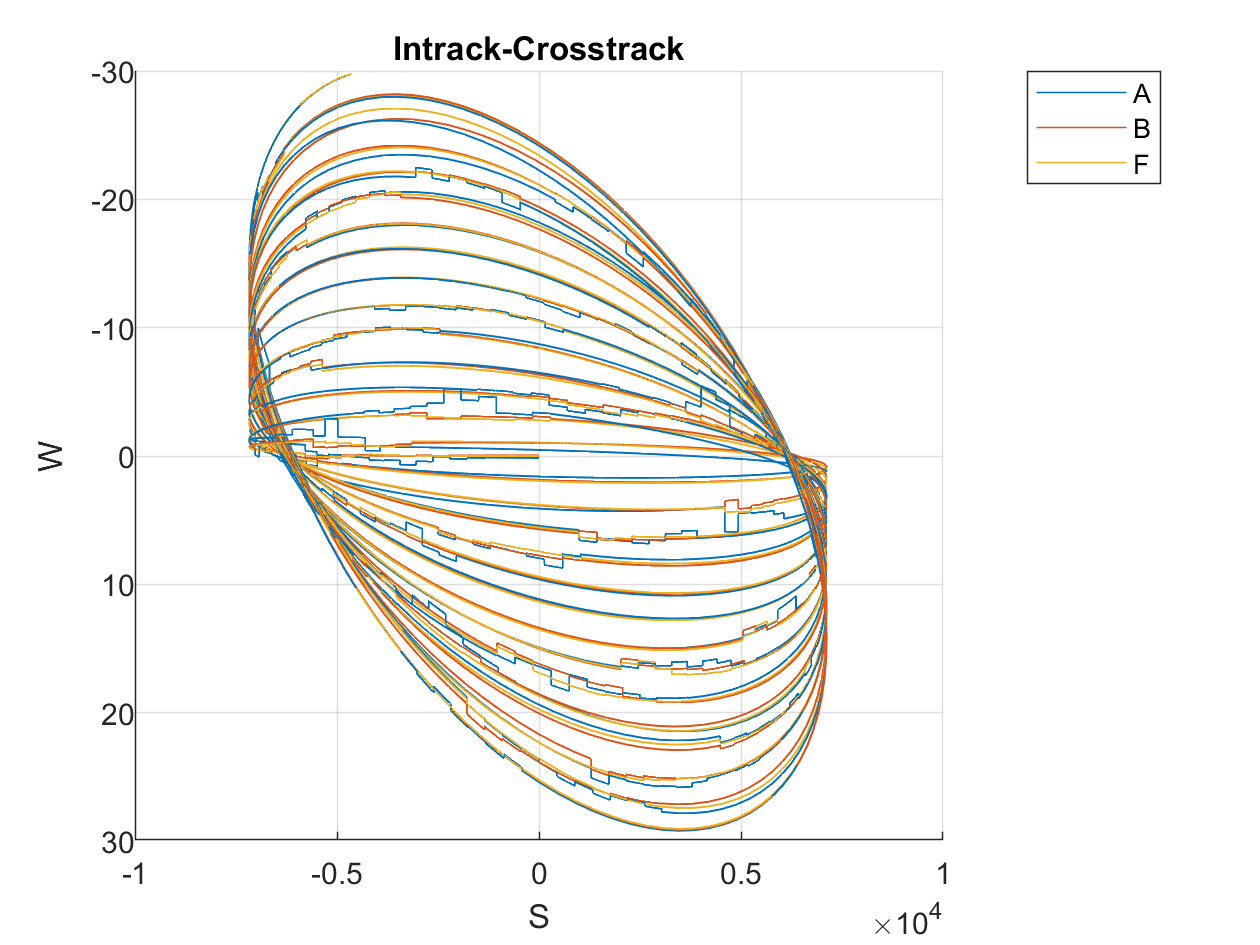
\includegraphics[width=0.6\textwidth]{intrack-crosstrackABF.png}
\end{center}

I suspect that something is going wrong with the station-only estimation and orbit propagation. 

\begin{table}[H]
	\begin{center}
	\begin{tabular}{|l|l|l|l|l|l|l|}
		\hline
		& Case A            & Case B           & Case C            & Case D           & Case E            & Case F            \\ \hline
		x (km) & -6330.33 & -6330.25  & -10041.40  & 1567.22  & -1924.64  & -6330.25 \\ \hline
		y (km) & 3306.96  & 3306.89   & 8472.56    & 4791.99  & -3742.66  & 3306.89  \\ \hline
		z (km) & 127.98   & 127.77    & 986.39     & 15103.25 & -1536.00  & 127.82   \\ \hline
	\end{tabular}
\caption{Predicted Position of JahSat after 24 hours in ECI frame}
\end{center}
\end{table}

When the final best estimate of Case F is converted into orbital elements, the eccentricity is 0.00403122939916287. That is quite circular, which possibly indicates to me that the satellite is either nearing the end of orbit raising and nearing its final orbital position, or is about to be raised into a graveyard orbit as a delta-V maneuver is planned at 24 hours. 

For my orbit determination process I am using a [6x1] state vector composed of satellite position and velocity in ECI frame. I am working with units in kilometers and kilometers/second. My dynamics include 20x20 spherical harmonics gravity field, lunisolar perturbations, SRP modeled as pressure on the solar panel, and cannonball drag. 

I then used a batch filter to refine the initial condition. The batch filter was initialized with the following station noise errors (converted into km and km/s in the code):

\begin{table}[H]
	\begin{center}
		\begin{tabular}{|l|l|l|l|}
			\hline 
			Number & Description & Range $\sigma$ (m) & Range Rate $\sigma$ (mm) \\ \hline 
			1 & Kwajalein & 10 & 0.5 \\ \hline 
			2 & Diego Garcia & 5 & 1 \\ \hline 
			3 & Arecibo & 10 & 0.5 \\ \hline 
		\end{tabular}
	\end{center}
\end{table} 

The state covariance was initialized for position error for 10 km and velocity error of 10 m/s: 

\begin{equation*}
	P_0 = 
	\begin{bmatrix}
		10^2I_{3x3} & 0_{3x3} \\
		0_{3x3} & (10^{-3})^2I_{3x3} 
	\end{bmatrix}
\end{equation*}

The algorithm for the Batch filter was taken from Born, Section 4.6: Computational Algorithm for the Batch Processor \cite{born_statorbitdet}. The first 28 measurements were iterated in the batch filter until the updated state changed by less than 0.1 m. 

Then, I used an Extended Kalman Filter to filter and update the best estimate of the trajectory, which also taken from Born, Section 4.7.3: The Extended Sequential Computational Algorithm. The last updated covariances from the batch filter were used to initialize the EKF. The prefit residuals were computed using the dynamically propagated state, and the postfit residuals were computed using the measurement-updated state. 

For the range and range-only simulations, I updated the EKF to use a reduced dimension G matrix (mapping of state space to measurement space). The observation-state H matrix was also updated to reflect range or range-only measurements. 

The process noise Q was initially set at 1e-20 along the diagonal, but the estimate improved vastly when I increased the power. I saw no better performance past 1e-12 for the diagonal elements and I didn't want to jack up the process noise too much to cover my modeling sins. For the next phase of the project, I am planning on including light-time correction. 




\newpage
% ================================================================ % 
\section*{Appendix} 

\subsection*{HW5 MATLAB code} 

\textbf{Note: The equations of motion and functions to transform from ECI to ECEF and back were submitted as part of Homework 4, and so are left out of this appendix.}

\textbf{finalproj\_EOM\_batch.m:}
\begin{lstlisting}[basicstyle=\footnotesize]
% HW 5 
% Junette Hsin 

clear; clc 
addpath(genpath('mice')); 
addpath(genpath('spice_data')); 

% Load SPICE kernel file 
cspice_furnsh( 'spice_data/naif0011.tls' )
cspice_furnsh( 'spice_data/de421.bsp' )       
cspice_furnsh( 'spice_data/pck00010.tpc ') 

format long g 

%% Parameters 

global muE RE muS AU muM eE wE J2 J3 J4 Cd Cs eop_data 
global A m p p0 r0_drag H CD

% initial state initial guess (M --> KM)
CD  = 1.88;    
X0 = [ 6984.45711518852 
1612.2547582643 
13.0925904314402 
-1.67667852227336
7.26143715396544
0.259889857225218 ]; 

% ballpark right answer 
% X0 = [  6978.25607108059
%         1616.30079732436
%         19.7187784486054
%        -1.66208620583392
%         7.26104892573667
%         0.270612926043287 ]; 

nX  = length(X0); 

% initialize STM 
STM0 = eye(length(X0)); 
STM0 = reshape(STM0, [length(X0)^2 1]); 
XSTM0 = [X0; STM0];  

% Constants 
muE = 398600.4415;          % Earth Gravitational Parameter (km^3/s^2) 
RE  = 6378.1363;            % Earth Radius (km)
muS = 132712440018;         % Sun's Gravitational Parameter (km^3/s^2)
AU  = 149597870.7;          % 1 Astronomical Unit (km)
muM = 4902.800066;          % Moon's Gravitational Parameter (km^3/s^2)
eE  = 0.081819221456;       % Earth's eccentricity 
wE  = 7.292115146706979e-5; % Earth's rotational velocity (rad/s)
m   = 2000;                 % satellite mass (kg) 
Cd  = 0.04;                 % diffuse reflection 
Cs  = 0.04;                 % specular reflection 

J2 = 1.08262617385222e-3; 
J3 = -2.53241051856772e-6;
J4 = -1.61989759991697e-6; 

global r_KJL_ECEF r_DGO_ECEF r_ACB_ECEF 

% Station coords. Convert M --> KM 
r_KJL_ECEF = [-6143584  1364250  1033743]' / 1000;  % Kwajalein 
r_DGO_ECEF = [ 1907295  6030810 -817119 ]' / 1000;  % Diego 
r_ACB_ECEF = [ 2390310 -5564341  1994578]' / 1000;  % Arecibo 

global LEO_DATA_Apparent 
% Load observation data 
load('LEO_DATA_Apparent.mat') 

% Station data 
ID_STA   = 1; 
i_STA    = find(LEO_DATA_Apparent(:, 1) == ID_STA); 
Yobs_KJL = LEO_DATA_Apparent(i_STA, :); 
t_KWJ    = Yobs_KJL(:,2); 

ID_STA   = 2; 
i_STA    = find(LEO_DATA_Apparent(:, 1) == ID_STA); 
Yobs_DGO = LEO_DATA_Apparent(i_STA, :);
t_DGO    = Yobs_DGO(:,2); 

ID_STA   = 3; 
i_STA    = find(LEO_DATA_Apparent(:, 1) == ID_STA); 
Yobs_ACB = LEO_DATA_Apparent(i_STA, :);
t_ACB    = Yobs_DGO(:,2); 

eop_data = load('finals_iau1980.txt'); 

% Atmospheric drag 
r   = norm(X0(1:3));            % km 
H   = 88667.0 / 1000;           % m --> km 
r0_drag  = (700 + RE);          % m --> km 
p0  = 3.614e-13 * 1e9;          % kg/m3 --> kg/km^3 
p   = p0*exp( -(r-r0_drag)/H ); 
A   = 15 / 1e6;                 % km^2 

global Cnm Snm 

% Gravity 
Cnm = zeros(181,181);
Snm = zeros(181,181);
fid = fopen('GGM03S.txt','r');
for n=0:180
for m=0:n
temp = fscanf(fid,'%d %d %f %f %f %f',[6 1]);        
Cnm(n+1,m+1) = temp(3);
Snm(n+1,m+1) = temp(4);
end
end

%% Convert t0 to ET, i.e. seconds past J2000, the base time variable for SPICE. function calls.

%  Epoch for initial conditions 
% epoch = 23 March 2018, 08:55:03 UTC ; 
t0      = 'March 23, 2018, 08:55:03 UTC'; 
abcorr  = 'NONE';

%  Convert the epoch to ephemeris time. 
et_t0   = cspice_str2et( t0 );

% extract observation epochs 
epochs = LEO_DATA_Apparent(:,2); 
epochs = et_t0 + epochs; 


%% Derive A and H matrices 

X  = sym('X', [length(X0) 1]); 
dX = fn.EOM(et_t0, X); 

% compute partials 
Amat    = jacobian( dX, X );       
Amat_fn = matlabFunction(Amat); 

% DO EVERYTHING IN ECI FRAME 

X  = sym('X', [nX; 1]); 
XS = sym('XS', [nX; 1]); 

r_site = [X(1)-XS(1); X(2)-XS(2); X(3)-XS(3)]; 
v_site = [X(4)-XS(4); X(5)-XS(5); X(6)-XS(6)]; 
d      = norm(r_site); 
v      = dot(v_site, r_site/norm(r_site)); 

Htmat      = sym(zeros(2,nX)); 
Htmat(1,:) = simplify(gradient(d, X)); 
Htmat(2,:) = simplify(gradient(v, X)); 
Ht_fn      = matlabFunction(Htmat); 

Ht_r_fn  = matlabFunction(Htmat(1,:)); 
Ht_rr_fn = matlabFunction(Htmat(2,:)); 

%% integrate EOM 

% set ode45 params 
rel_tol = 1e-10;         % 1e-14 accurate; 1e-6 coarse 
abs_tol = 1e-10; 
options = odeset('reltol', rel_tol, 'abstol', abs_tol ); 

% Set run state 
run_state = 2; 
disp('Running sim ...') 

if run_state == 1
[t, X] = ode45(@fn.EOM, [epochs(1) : 60 : epochs(end)], X0, options); 
elseif run_state == 2
[t, XSTM] = ode45(@(t, XSTM) fn.EOM_STM(t, XSTM, Amat_fn, nX), [epochs(1) : 60 : epochs(end)], XSTM0, options); 
X = XSTM(:, 1:6); 
end 
disp('Pos and Vel end: ')
disp(X(end, 1:6)'); 

XSTM_ref0   = XSTM; 
t_XSTM_ref0 = t; 


%% Setting up filters 

% weighting matrices m --> km, mm --> km 
global R_KJL R_DGO R_ACB 
R_KJL = [(10e-3)^2 0; 0 (0.5e-6)^2]; 
R_DGO = [(5e-3)^2  0; 0 (1e-6)^2]; 
R_ACB = [(10e-3)^2 0; 0 (0.5e-6)^2]; 

% initial covariance error 
% 10 km std - position 
% 10 m/s    - velocity 
P0 = [ 10^2*eye(3), zeros(3); 
zeros(3),  (10e-3)^2*eye(3) ]; 
Lambda0 = inv(P0); 
global Lambda_KJL0 Lambda_DGO0 Lambda_ACB0
Lambda_KJL0 = Lambda0; 
Lambda_DGO0 = Lambda0; 
Lambda_ACB0 = Lambda0; 

global N_KJL0 N_DGO0 N_ACB0
N0    = Lambda0*X0; 
N_KJL0 = N0; 
N_DGO0 = N0; 
N_ACB0 = N0; 


%% Batch all stations to refine IC 

Xstar  = 100*ones(1,3); 
XSTM   = XSTM_ref0; 
t_XSTM = t_XSTM_ref0; 
XSTM0  = XSTM_ref0(1,:)'; 
iter   = 0; 
N_prev = N0; 
Lambda_prev = Lambda0; 

% Batch first 28 measurements 

while norm(Xstar(1:3)) > 0.1

% keep track of iterations 
iter = iter + 1; 
sprintf('iter = %d', iter)

% Test - All stations 
[Ycalc_all, Lambda, N] = ... 
fn.batch_LSQ(LEO_DATA_Apparent, t_XSTM, XSTM, et_t0, Ht_fn, Lambda_prev, N_prev); 

%     % Test - Kwajalein 
%     [Ycalc_all, Lambda, N] = ... 
%         fn.batch_LSQ(Yobs_KJL, t_XSTM, XSTM, et_t0, Ht_fn, Lambda0, N0); 

% Solve normal equation 
Xstar = inv(Lambda) * N; 

% update covariance 
Lambda_prev = Lambda0; 
N_prev      = N0; 

% update initial conditions 
XSTM0(1:nX) = XSTM0(1:nX) + Xstar; 
[t, XSTM] = ode45(@(t, XSTM) fn.EOM_STM(t, XSTM, Amat_fn, nX), [epochs(1) : 60 : epochs(end)], XSTM0, options); 

disp('xhat pos'); Xstar(1:3)
disp('xhat pos norm'); norm(Xstar(1:3))
disp('x IC pos'); XSTM0(1:3)

end 

Lambda_batch = Lambda; 
XSTM_batch   = XSTM; 
XSTM0_batch  = XSTM0; 
\end{lstlisting}

\textbf{finalproj\_EKF.m:}
\begin{lstlisting}
% HW 5 
% Junette Hsin 

% finalproj_EOM_batch; 

%% EKF - all observations 

STATIONS = 0; 
% for STATIONS = 1:3 
for DATA = 1:2

%         DATA = 0; 
if STATIONS == 0    % use all station data 
Yobs_STA = LEO_DATA_Apparent; 
elseif STATIONS == 1 
Yobs_STA = Yobs_KJL; 
elseif STATIONS == 2
Yobs_STA = Yobs_DGO;     
else % STATIONS == 3
Yobs_STA = Yobs_ACB;
end 

et_obs     = Yobs_STA(:,2) + et_t0; 
XSTM_prev  = XSTM0_batch; 

iter       = 0; 
P_prev     = inv(Lambda_batch);

X_EKF      = []; 
t_X_EKF    = []; 
Y_prefit   = []; 
Y_postfit  = []; 

Lambda_mat = []; 
sigma3     = []; 

for i = 1:length(et_obs)

% keep track of iterations 
iter = iter + 1; 
sprintf('iter = %d', iter)

% Propagate state 
if     i == 1 && et_obs(1) == et_t0; t_prop = et_obs(i); 
elseif i == 1;                       t_prop = [et_t0 : 60 : et_obs(1) ]; 
else;                                t_prop = [et_obs(i-1) : 60 : et_obs(i)]; 
end

% EKF. All data, range, or range-only 
if DATA == 0
[t_XSTM, XSTM, Xstar, Y_pre, Y_post, P, Lambda] = fn.EKF(Yobs_STA, XSTM_prev, nX, ... 
epochs(1), t_prop, options, Amat_fn, Ht_fn, P_prev); 
elseif DATA == 1
% EKF for range only 
[t_XSTM, XSTM, Xstar, Y_pre, Y_post, P, Lambda] = fn.EKF_r(Yobs_STA, XSTM_prev, nX, ... 
epochs(1), t_prop, options, Amat_fn, Ht_r_fn, P_prev); 
else % DATA == 2
% EKF for range-rate only 
[t_XSTM, XSTM, Xstar, Y_pre, Y_post, P, Lambda] = fn.EKF_rr(Yobs_STA, XSTM_prev, nX, ... 
epochs(1), t_prop, options, Amat_fn, Ht_rr_fn, P_prev); 
end

% save states from current iteration 
if i == 1 && et_obs(1) == et_t0; X_EKF = XSTM(1:nX)'; 
else;                            X_EKF = [X_EKF; XSTM(:, 1:nX)]; 
end 

t_X_EKF   = [t_X_EKF; t_XSTM]; 
Y_prefit  = [Y_prefit; Y_pre]; 
Y_postfit = [Y_postfit; Y_post]; 

% update measurement for next iteration 
XSTM_prev = [Xstar; STM0]; 
P_prev    = P;

% innovations covariance 
Lambda_mat = [Lambda_mat; Lambda]; 

% 3-sigma STD 
if DATA == 0; sigma3 = [sigma3; sqrt(Lambda(1,1))*3, sqrt(Lambda(2,2))*3];  
else;         sigma3 = [sigma3; sqrt(Lambda(1,1))*3];  
end

end 

% Propagate to last period of time 
t_prop = [ et_obs(end) : 60 : et_t0 + 60*60*24 ]; 
[t_XSTM, XSTM] = ode45(@(t, XSTM) fn.EOM_STM(t, XSTM, Amat_fn, nX), t_prop, XSTM_prev, options); 
Xi   = XSTM(end,1:nX)'; 
STMi = XSTM(end,nX+1:end); 
STMi = reshape(STMi, [nX nX]); 

% Time update + process noise 
dt    = t_prop(end) - t_prop(1); 
Q     = diag( (10000e-10)^2 * [1 1 1] ); 
Gamma = [diag( dt^2/2 * [1 1 1] ); diag([dt dt dt])]; 
P_noise = Gamma * Q * Gamma'; 
Pi_bar = STMi * P_prev * STMi' + P_noise; 

X_EKF_prop   = [X_EKF; XSTM(:,1:nX)]; 
t_X_EKF_prop = [t_X_EKF; t_XSTM]; 


%% Plot satellite position 

ftitle = 'JahSat Orbit'; 
figure('name', ftitle); 
plot3(XSTM_ref0(:,1), XSTM_ref0(:,2), XSTM_ref0(:,3)); hold on; grid on; 
plot3(XSTM_batch(:,1), XSTM_batch(:,2), XSTM_batch(:,3)); 
plot3(X_EKF(:,1), X_EKF(:,2), X_EKF(:,3)); hold on; grid on; 
plot3(X_EKF(1,1), X_EKF(1,2), X_EKF(1,3), 'o')
xlabel('x (km)'); ylabel('y (km)'); zlabel('z (km)'); 
legend('initial', 'batch', 'EKF', 'prop') 
title(ftitle)


%% Calculate residuals 

Ypre_KJL = [];      Ypre_DGO = [];      Ypre_ACB = []; 

Ypost_KJL = [];     Ypost_DGO = [];     Ypost_ACB = []; 

sigma3_KJL = [];    sigma3_DGO = [];    sigma3_ACB = []; 

% Extract states that correspond with station measurements 
for i = 1:length(Y_postfit)

ti  = Y_postfit(i, 2); 
ti  = ti + et_t0; 
i_X = find(t_X_EKF == ti); 

i_STA = Y_postfit(i, 1); 

if i_STA == 1
Ypre_KJL   = [Ypre_KJL; Y_prefit(i,:)]; 
Ypost_KJL  = [Ypost_KJL; Y_postfit(i,:)]; 
sigma3_KJL = [sigma3_KJL; sigma3(i,:)]; 
elseif i_STA == 2
Ypre_DGO   = [Ypre_DGO; Y_prefit(i,:)]; 
Ypost_DGO  = [Ypost_DGO; Y_postfit(i,:)]; 
sigma3_DGO = [sigma3_DGO; sigma3(i,:)]; 
else
Ypre_ACB   = [Ypre_ACB; Y_prefit(i,:)]; 
Ypost_ACB  = [Ypost_ACB; Y_postfit(i,:)]; 
sigma3_ACB = [sigma3_ACB; sigma3(i,:)]; 
end 

end 

t_KJL = Yobs_KJL(:,2); 
t_DGO = Yobs_DGO(:,2); 
t_ACB = Yobs_ACB(:,2); 

if STATIONS == 0
if DATA == 0
res_all_plot_STA(t_KJL, Yobs_KJL, Ypre_KJL, Ypost_KJL, sigma3_KJL, 'Kwajalein Residuals'); 
res_all_plot_STA(t_DGO, Yobs_DGO, Ypre_DGO, Ypost_DGO, sigma3_DGO, 'Diego-Garcia Residuals'); 
res_all_plot_STA(t_ACB, Yobs_ACB, Yobs_ACB, Yobs_ACB, sigma3_ACB, 'Arecibo Residuals'); 
elseif DATA == 1
res_r_plot_STA(t_KJL, Yobs_KJL, Ypre_KJL, Ypost_KJL, sigma3_KJL, 'Kwajalein Residuals (Range Only)')
res_r_plot_STA(t_DGO, Yobs_DGO, Ypre_DGO, Ypost_DGO, sigma3_DGO, 'Diego-Garcia Residuals (Range Only)')
res_r_plot_STA(t_ACB, Yobs_ACB, Ypre_ACB, Ypost_ACB, sigma3_ACB, 'Arecibo Residuals (Range Only)')
else
res_rr_plot_STA(t_KJL, Yobs_KJL, Ypre_KJL, Ypost_KJL, sigma3_KJL, 'Kwajalein Residuals (Range-Rate Only)')
res_rr_plot_STA(t_DGO, Yobs_DGO, Ypre_DGO, Ypost_DGO, sigma3_DGO, 'Diego-Garcia Residuals (Range-Rate Only)')
res_rr_plot_STA(t_ACB, Yobs_ACB, Ypre_ACB, Ypost_ACB, sigma3_ACB, 'Arecibo Residuals (Range-Rate Only)')
end
elseif STATIONS == 1
res_all_plot_STA(t_KJL, Yobs_KJL, Ypre_KJL, Ypost_KJL, sigma3_KJL, 'Kwajalein Residuals'); 
elseif STATIONS == 2
res_all_plot_STA(t_DGO, Yobs_DGO, Ypre_DGO, Ypost_DGO, sigma3_DGO, 'Diego-Garcia Residuals'); 
else % STATIONS == 3
res_all_plot_STA(t_ACB, Yobs_ACB, Yobs_ACB, Yobs_ACB, sigma3_ACB, 'Arecibo Residuals'); 
end 


%% radial-intrack-cross-track frame transformation for best estimate 

% radial-intrack-cross-track frame transformation for best estimate 
if STATIONS == 0  && DATA == 0 
T_best = fn.ECItoRSW_T(Xi); 
end 

% transform all measurements 
X_RSW = []; 
for i = 1:length(X_EKF_prop) 
X_RSW = [ X_RSW; [T_best * X_EKF_prop(i, 1:3)']' ]; 
end 

if STATIONS == 0
if DATA == 0
X_ALL_RSW = X_RSW; 
save('X_ALL_RSW.mat') 
elseif DATA == 1
X_R_RSW = X_RSW; 
save('X_R_RSW.mat') 
else
X_RR_RSW = X_RSW; 
save('X_RR_RSW.mat') 
end
elseif STATIONS == 1
X_KJL_RSW = X_RSW; 
save('X_KJL_RSW.mat') 
elseif STATIONS == 2
X_DGO_RSW = X_RSW; 
save('X_DGO_RSW.mat') 
else
X_ACB_RSW = X_RSW; 
save('X_ACB_RSW.mat') 
end 

%     end
end

%% Plot radial-intrack-crosstrack 

% Start figure 
ftitle = 'Radial-Intrack-Crosstrack'; 
figh = figure('name', ftitle); 
plot3(X_R_RSW(:,1), X_R_RSW(:,2), X_R_RSW(:,3)); hold on; grid on;  
plot3(X_RR_RSW(:,1), X_RR_RSW(:,2), X_RR_RSW(:,3)); 
%     plot3(X_KJL_RSW(:,1), X_KJL_RSW(:,2), X_KJL_RSW(:,3)); 
%     plot3(X_DGO_RSW(:,1), X_DGO_RSW(:,2), X_DGO_RSW(:,3)); 
%     plot3(X_ACB_RSW(:,1), X_ACB_RSW(:,2), X_ACB_RSW(:,3)); 
plot3(X_ALL_RSW(:,1), X_ALL_RSW(:,2), X_ALL_RSW(:,3)); 
%     legend('A', 'B', 'C', 'D', 'E', 'F') 
legend('A', 'B', 'F') 
xlabel('R')
ylabel('S') 
zlabel('W') 


%% Subfunctions 

function res_all_plot_STA(t_KJL, Yobs_KJL, Ypre_KJL, Ypost_KJL, sigma3_KJL, ftitle)

[dpre_err_KJL, dpre_rms_KJL, vpre_err_KJL, vpre_rms_KJL] = calc_res_all(Yobs_KJL, Ypre_KJL); 
[dpost_err_KJL, dpost_rms_KJL, vpost_err_KJL, vpost_rms_KJL] = calc_res_all(Yobs_KJL, Ypost_KJL); 

plot_res_all(ftitle, t_KJL, sigma3_KJL, dpre_err_KJL, dpre_rms_KJL, vpre_err_KJL, vpre_rms_KJL, ... 
dpost_err_KJL, dpost_rms_KJL, vpost_err_KJL, vpost_rms_KJL)

end 

function res_r_plot_STA(t_KJL, Yobs_KJL, Ypre_KJL, Ypost_KJL, sigma3_KJL, ftitle)

[dpre_err_KJL, dpre_rms_KJL]   = calc_res_r(Yobs_KJL, Ypre_KJL); 
[dpost_err_KJL, dpost_rms_KJL] = calc_res_r(Yobs_KJL, Ypost_KJL); 

plot_res_r(ftitle, t_KJL, sigma3_KJL, dpre_err_KJL, dpre_rms_KJL, dpost_err_KJL, dpost_rms_KJL)

end 

function res_rr_plot_STA(t_KJL, Yobs_KJL, Ypre_KJL, Ypost_KJL, sigma3_KJL, ftitle)

[vpre_err_KJL, vpre_rms_KJL]   = calc_res_rr(Yobs_KJL, Ypre_KJL); 
[vpost_err_KJL, vpost_rms_KJL] = calc_res_rr(Yobs_KJL, Ypost_KJL); 

plot_res_r(ftitle, t_KJL, sigma3_KJL, vpre_err_KJL, vpre_rms_KJL, vpost_err_KJL, vpost_rms_KJL)

end 

function [d_err_STA, d_rms_STA, v_err_STA, v_rms_STA] = calc_res_all(Yobs_STA, Ycalc_STA)

% Calculate residuals 
d_err_STA = Yobs_STA(:,3) - Ycalc_STA(:,3); 
d_rms_STA = rms(d_err_STA); 
v_err_STA = Yobs_STA(:,4) - Ycalc_STA(:,4); 
v_rms_STA = rms(v_err_STA); 

end 

function [d_err_STA, d_rms_STA] = calc_res_r(Yobs_STA, Ycalc_STA)

% Calculate residuals 
d_err_STA = Yobs_STA(:,3) - Ycalc_STA(:,3); 
d_rms_STA = rms(d_err_STA); 

end 

function [v_err_STA, v_rms_STA] = calc_res_rr(Yobs_STA, Ycalc_STA)

% Calculate residuals 
v_err_STA = Yobs_STA(:,4) - Ycalc_STA(:,3); 
v_rms_STA = rms(v_err_STA); 

end 

function plot_res_all(ftitle, t_STA, sigma3_STA, dpre_err_STA, dpre_rms_STA, vpre_err_STA, vpre_rms_STA, ... 
dpost_err_STA, dpost_rms_STA, vpost_err_STA, vpost_rms_STA)

figure('name', ftitle); 
subplot(4,1,1) 
scatter(t_STA, dpre_err_STA); hold on; grid on; 
title({sprintf('PREFIT range residuals (km): mean = %.3g, RMS = %.3g', mean(dpre_err_STA), dpre_rms_STA)} ); 
	ylabel('km')  
	subplot(4,1,2) 
	scatter(t_STA, vpre_err_STA); hold on; grid on; 
	title({sprintf('PREFIT range-rate residuals (km/s): mean = %.3g, RMS = %.3g', mean(vpre_err_STA), vpre_rms_STA)} ); 
		xlabel('Time (s)') 
		ylabel('km/s') 
		subplot(4,1,3) 
		scatter(t_STA, dpost_err_STA); hold on; grid on; 
		plot(t_STA, sigma3_STA(:,1), 'r'); 
		plot(t_STA, -sigma3_STA(:,1), 'r'); 
		title({sprintf('POSTFIT range residuals (km): mean = %.3g, RMS = %.3g', mean(dpost_err_STA), dpost_rms_STA)} ); 
			ylabel('km')  
			subplot(4,1,4) 
			scatter(t_STA, vpost_err_STA); hold on; grid on; 
			plot(t_STA, sigma3_STA(:,2), 'r'); 
			plot(t_STA, -sigma3_STA(:,2), 'r'); 
			title({sprintf('POSTFIT range-rate residuals (km/s): mean = %.3g, RMS = %.3g', mean(vpost_err_STA), vpost_rms_STA)} ); 
				xlabel('Time (s)') 
				ylabel('km/s') 
				sgtitle(ftitle); 
				
				end 
				
				function plot_res_r(ftitle, t_STA, sigma3_STA, dpre_err_STA, dpre_rms_STA, dpost_err_STA, dpost_rms_STA)
				
				figure('name', ftitle); 
				subplot(2,1,1) 
				scatter(t_STA, dpre_err_STA); hold on; grid on; 
				title({sprintf('PREFIT range residuals (km): mean = %.3g, RMS = %.3g', mean(dpre_err_STA), dpre_rms_STA)} ); 
					ylabel('km')  
					subplot(2,1,2) 
					scatter(t_STA, dpost_err_STA); hold on; grid on; 
					plot(t_STA, sigma3_STA(:,1), 'r'); 
					plot(t_STA, -sigma3_STA(:,1), 'r'); 
					title({sprintf('POSTFIT range residuals (km): mean = %.3g, RMS = %.3g', mean(dpost_err_STA), dpost_rms_STA)} ); 
						ylabel('km')  
						sgtitle(ftitle); 
						
						end 
						
						function plot_res_rr(ftitle, t_STA, sigma3_STA, vpre_err_STA, vpre_rms_STA, vpost_err_STA, vpost_rms_STA)
						
						figure('name', ftitle); 
						subplot(2,1,1) 
						scatter(t_STA, vpre_err_STA); hold on; grid on; 
						title({sprintf('PREFIT range-rate residuals (km/s): mean = %.3g, RMS = %.3g', mean(vpre_err_STA), vpre_rms_STA)} ); 
							ylabel('km')  
							subplot(2,1,2) 
							scatter(t_STA, vpost_err_STA); hold on; grid on; 
							plot(t_STA, sigma3_STA(:,1), 'r'); 
							plot(t_STA, -sigma3_STA(:,1), 'r'); 
							title({sprintf('POSTFIT range-rate residuals (km/s): mean = %.3g, RMS = %.3g', mean(vpost_err_STA), vpost_rms_STA)} ); 
								ylabel('km')  
								sgtitle(ftitle); 
								
								end
\end{lstlisting}

\textbf{batch\_LSQ.m:}
\begin{lstlisting}
function [Ycalc_STA, Lambda, N] = ... 
batch_LSQ(Yobs_STA, t_XSTM, XSTM, et_t0, Ht_fn, Lambda0, N0)

global wE R_KJL R_DGO R_ACB 
global r_KJL_ECEF r_DGO_ECEF r_ACB_ECEF 

% Initialize calculated Y 
Ycalc_STA = zeros(size(Yobs_STA)); 
Ycalc_STA(:, 1:2) = Yobs_STA(:, 1:2); 

% Set up covariance 
nX     = length(N0); 
Lambda = Lambda0; 
N      = N0; 

% for i = 1:length(Yobs_STA)
for i = 1:28

% find index for same time state and observation 
Yi   = Yobs_STA(i, :); 
ti   = Yi(2) + et_t0; 
i_X  = find(t_XSTM == ti); 

% get JD time 
JD_UTC = cspice_et2utc(ti, 'J', 10); 
JD_UTC = str2num(extractAfter(JD_UTC, 'JD ')); 

% observation covariance 
if Yi(1) == 1
R = R_KJL; 
r_STA_ECEF = r_KJL_ECEF; 
elseif Yi(1) == 2
R = R_DGO; 
r_STA_ECEF = r_DGO_ECEF; 
else 
R = R_ACB; 
r_STA_ECEF = r_ACB_ECEF; 
end 

% Convert station to ECI frame 
r_STA_ECI  = fn.ECEFtoECI(JD_UTC, r_STA_ECEF); 
v_KJL_ECEF = [0; 0; 0]; 
a_ECEF     = v_KJL_ECEF + cross([ 0 0 wE ]', r_STA_ECEF); 
v_STA_ECI  = fn.ECEFtoECI(JD_UTC, a_ECEF); % Technically wrong. Look in Vallado 
XSi        = [r_STA_ECI; v_STA_ECI]; 

% Extract states (all in ECI) 
Xi   = XSTM( i_X, 1:nX)'; 
STMi = XSTM( i_X, nX+1 : nX+nX^2 ); 
STMi = reshape(STMi, [nX nX]); 

% compute H [2x7]
Hi = Ht_fn(Xi(1), Xi(2), Xi(3), Xi(4), Xi(5), Xi(6), XSi(1), XSi(2), XSi(3), XSi(4), XSi(5), XSi(6)) * STMi; 

% Accumulate observation 
Ycalc_STA(i,3:4) = Hi * Xi; 

% Obtain y difference 
yi = Yobs_STA(i,3:4)' - fn.G_fn(Xi, XSi); 

% Accumulate covariance 
Lambda = Lambda + Hi' * inv(R) * Hi; 
N      = N + Hi' * inv(R) * yi; 

end 

end 
\end{lstlisting}

\textbf{EKF.m:}
\begin{lstlisting}
function [t_XSTM, XSTM, Xstar, Y_prefit, Y_postfit, Pi, Lambda] = ... 
EKF(Yobs_STA, XSTM_prev, nX, et_t0, t_prop, options, Amat_fn, Ht_fn, P_prev)

global wE R_KJL R_DGO R_ACB 
global r_KJL_ECEF r_DGO_ECEF r_ACB_ECEF 

% Integrate ref trajectory and STM from t = i-1 (prev) to t = i (curr) 
if length(t_prop) > 1
[t_XSTM, XSTM] = ode45(@(t, XSTM) fn.EOM_STM(t, XSTM, Amat_fn, nX), t_prop, XSTM_prev, options); 
Xi   = XSTM(end,1:nX)'; 
STMi = XSTM(end,nX+1:end); 
else
t_XSTM = t_prop; 
XSTM = XSTM_prev; 
Xi   = XSTM(1:nX); 
STMi = XSTM(nX+1:end); 
end 
STMi = reshape(STMi, [nX nX]); 

% % find index for same time state and observation 
t_Y   = Yobs_STA(:,2) + et_t0; % time after initial epoch 
ti_X  = t_XSTM(end); 
i_Y   = find(t_Y == ti_X); 
Yi    = Yobs_STA(i_Y, :); 

% get JD time 
JD_UTC = cspice_et2utc(t_XSTM(end), 'J', 10); 
JD_UTC = str2num(extractAfter(JD_UTC, 'JD ')); 

% observation covariance 
if Yi(1) == 1
R = R_KJL; 
r_STA_ECEF = r_KJL_ECEF; 
elseif Yi(1) == 2
R = R_DGO; 
r_STA_ECEF = r_DGO_ECEF; 
else 
R = R_ACB; 
r_STA_ECEF = r_ACB_ECEF; 
end 

% Convert station to ECI frame 
r_STA_ECI  = fn.ECEFtoECI(JD_UTC, r_STA_ECEF); 
v_KJL_ECEF = [0; 0; 0]; 
a_ECEF     = v_KJL_ECEF + cross([ 0 0 wE ]', r_STA_ECEF); 
v_STA_ECI  = fn.ECEFtoECI(JD_UTC, a_ECEF); % Technically wrong. Look in Vallado 
XSi        = [r_STA_ECI; v_STA_ECI]; 

% Time update + process noise 
dt    = t_prop(end) - t_prop(1); 
% Q     = diag( (1e-10)^2 * [1 1 1] ); 
Q     = diag( (10000e-10)^2 * [1 1 1] ); 
Gamma = [diag( dt^2/2 * [1 1 1] ); diag([dt dt dt])]; 
P_noise = Gamma * Q * Gamma'; 
Pi_bar = STMi * P_prev * STMi' + P_noise; 

% Y prefit 
Y_prefit(1:2) = Yi(1:2); 
Y_prefit(3:4) = fn.G_fn(Xi, XSi)'; 

% Observation-state matrix 
Hti = Ht_fn(Xi(1), Xi(2), Xi(3), Xi(4), Xi(5), Xi(6), XSi(1), XSi(2), XSi(3), XSi(4), XSi(5), XSi(6)); 

% Gain matrix 
Ki = Pi_bar * Hti' * inv( Hti * Pi_bar * Hti' + R ); 

% Obtain y difference 
yi = Yi(3:4)' - fn.G_fn(Xi, XSi); 

% Measurement and reference orbit update 
xhat  = Ki * yi; 
Xstar = Xi + xhat; 
Pi    = ( eye(nX) - Ki * Hti ) * Pi_bar;
% Pi    = ( eye(nX) - Ki * Hti ) * Pi_bar * ( eye(nX) - Ki * Hti )' + Ki * R * Ki'; 

% Innovation (information) covariance 
Lambda = (Hti * Pi * Hti' + R); 

% Y postfit 
Y_postfit(1:2) = Yi(1:2); 
Y_postfit(3:4) = fn.G_fn(Xstar, XSi)'; 

end 
\end{lstlisting}

\textbf{ECItoRSW\_t.m:}
\begin{lstlisting}
function T = ECItoRSW_T(X_ECI)

r_ECI = X_ECI(1:3); 
v_ECI = X_ECI(4:6); 

R = r_ECI / norm(r_ECI); 
W = cross(r_ECI, v_ECI) / norm(cross(r_ECI, v_ECI)); 
S = cross(W, R); 

T = [R'; S'; W']; 

end 
\end{lstlisting}


% ================================================================ % 

\bibliography{sample}

\end{document}
